% ============================================================
% ISEF POSTER — SURROGATE-ACCELERATED STRUCTURAL OPTIMIZATION
% 48 × 36 inch tri-fold | Matches Rishab Kumar Jain reference style
% Compile: lualatex poster.tex (or xelatex poster.tex)
% ============================================================
\documentclass[final]{beamer}
\usepackage[orientation=landscape, size=custom, width=121.92, height=91.44, scale=1.0]{beamerposter}
% 48in = 121.92cm, 36in = 91.44cm

% ── Packages ──────────────────────────────────────────────────
\usepackage{graphicx}
\usepackage{booktabs}
\usepackage{amsmath,amssymb}
\usepackage{enumitem}
\usepackage{multicol}
\usepackage{xcolor}
\usepackage{tikz}
\usetikzlibrary{calc,positioning,shapes.geometric,arrows.meta,decorations.pathreplacing}
\usepackage{fontspec}
\setmainfont{Arial}
\usepackage{ragged2e}
\usepackage{calc}
\usepackage{tcolorbox}
\tcbuselibrary{skins,breakable}
\usepackage{array}
\usepackage{tabularx}

% ── Color definitions ─────────────────────────────────────────
\definecolor{bgnavy}{HTML}{062B7A}
\definecolor{titleband}{HTML}{032061}
\definecolor{sectionbar}{HTML}{0A3D9A}
\definecolor{cardfill}{HTML}{F7F9FC}
\definecolor{cardborder}{HTML}{B7C5E3}
\definecolor{textdark}{HTML}{0B1736}
\definecolor{textwhite}{HTML}{FFFFFF}
\definecolor{accentred}{HTML}{D7263D}
\definecolor{accentteal}{HTML}{008C9E}
\definecolor{accentgold}{HTML}{CFA535}
\definecolor{eqpill}{HTML}{E8EEF8}
\definecolor{extwall}{HTML}{4A7FC1}
\definecolor{intwall}{HTML}{E8833A}
\definecolor{roofgreen}{HTML}{6AAF6E}

% ── Beamer theme config ───────────────────────────────────────
\setbeamercolor{background canvas}{bg=bgnavy}
\setbeamertemplate{navigation symbols}{}
\setbeamerfont{title}{size=\fontsize{62}{72}\selectfont, series=\bfseries}
\setbeamerfont{subtitle}{size=\fontsize{32}{38}\selectfont, series=\bfseries\itshape}
\setbeamerfont{author}{size=\fontsize{26}{32}\selectfont, series=\bfseries}

% ── Custom section header bar ─────────────────────────────────
\newtcolorbox{sectionbox}[1]{
    enhanced,
    colback=cardfill,
    colframe=cardborder,
    boxrule=0.5pt,
    arc=3pt,
    left=4pt, right=4pt, top=0pt, bottom=4pt,
    toptitle=3pt, bottomtitle=3pt,
    title={\centering\fontsize{24}{28}\selectfont\bfseries\color{white}\MakeUppercase{#1}},
    coltitle=white,
    colbacktitle=sectionbar,
    fonttitle=\bfseries,
    attach boxed title to top center={yshift=0pt},
    boxed title style={colback=sectionbar, colframe=sectionbar, arc=3pt, boxrule=0pt},
}

% ── Equation pill ─────────────────────────────────────────────
\newtcolorbox{eqbox}{
    enhanced,
    colback=eqpill,
    colframe=accentteal,
    boxrule=0.8pt,
    arc=4pt,
    left=8pt, right=8pt, top=4pt, bottom=4pt,
}

% ── Body text size ────────────────────────────────────────────
\newcommand{\bodytext}{\fontsize{13.5}{16}\selectfont\color{textdark}\justifying}
\newcommand{\captiontext}{\fontsize{11.5}{14}\selectfont\color{textdark}\itshape}
\newcommand{\subheader}[1]{\vspace{4pt}{\fontsize{16}{19}\selectfont\bfseries\color{textdark}#1}\vspace{2pt}\par}

% ============================================================
\begin{document}
\begin{frame}[t]

% ════════════════════════════════════════════════════════════════
% TITLE BAND (top 3.25 inches ≈ 8.26cm)
% ════════════════════════════════════════════════════════════════
\begin{tikzpicture}[remember picture, overlay]
    % Title band background
    \fill[titleband] (current page.north west) rectangle ([yshift=-8.26cm]current page.north east);
    % Gold rule at bottom of title band
    \draw[accentgold, line width=1.5pt] ([yshift=-8.2cm]current page.north west) -- ([yshift=-8.2cm]current page.north east);
    
    % Left element placeholder (house render)
    \node[anchor=north west, inner sep=0] at ([xshift=1cm, yshift=-0.5cm]current page.north west) {
        \colorbox{titleband}{%
            \begin{minipage}{12cm}
                \centering
                \vspace{0.5cm}
                {\fontsize{11}{13}\selectfont\color{white}\itshape
                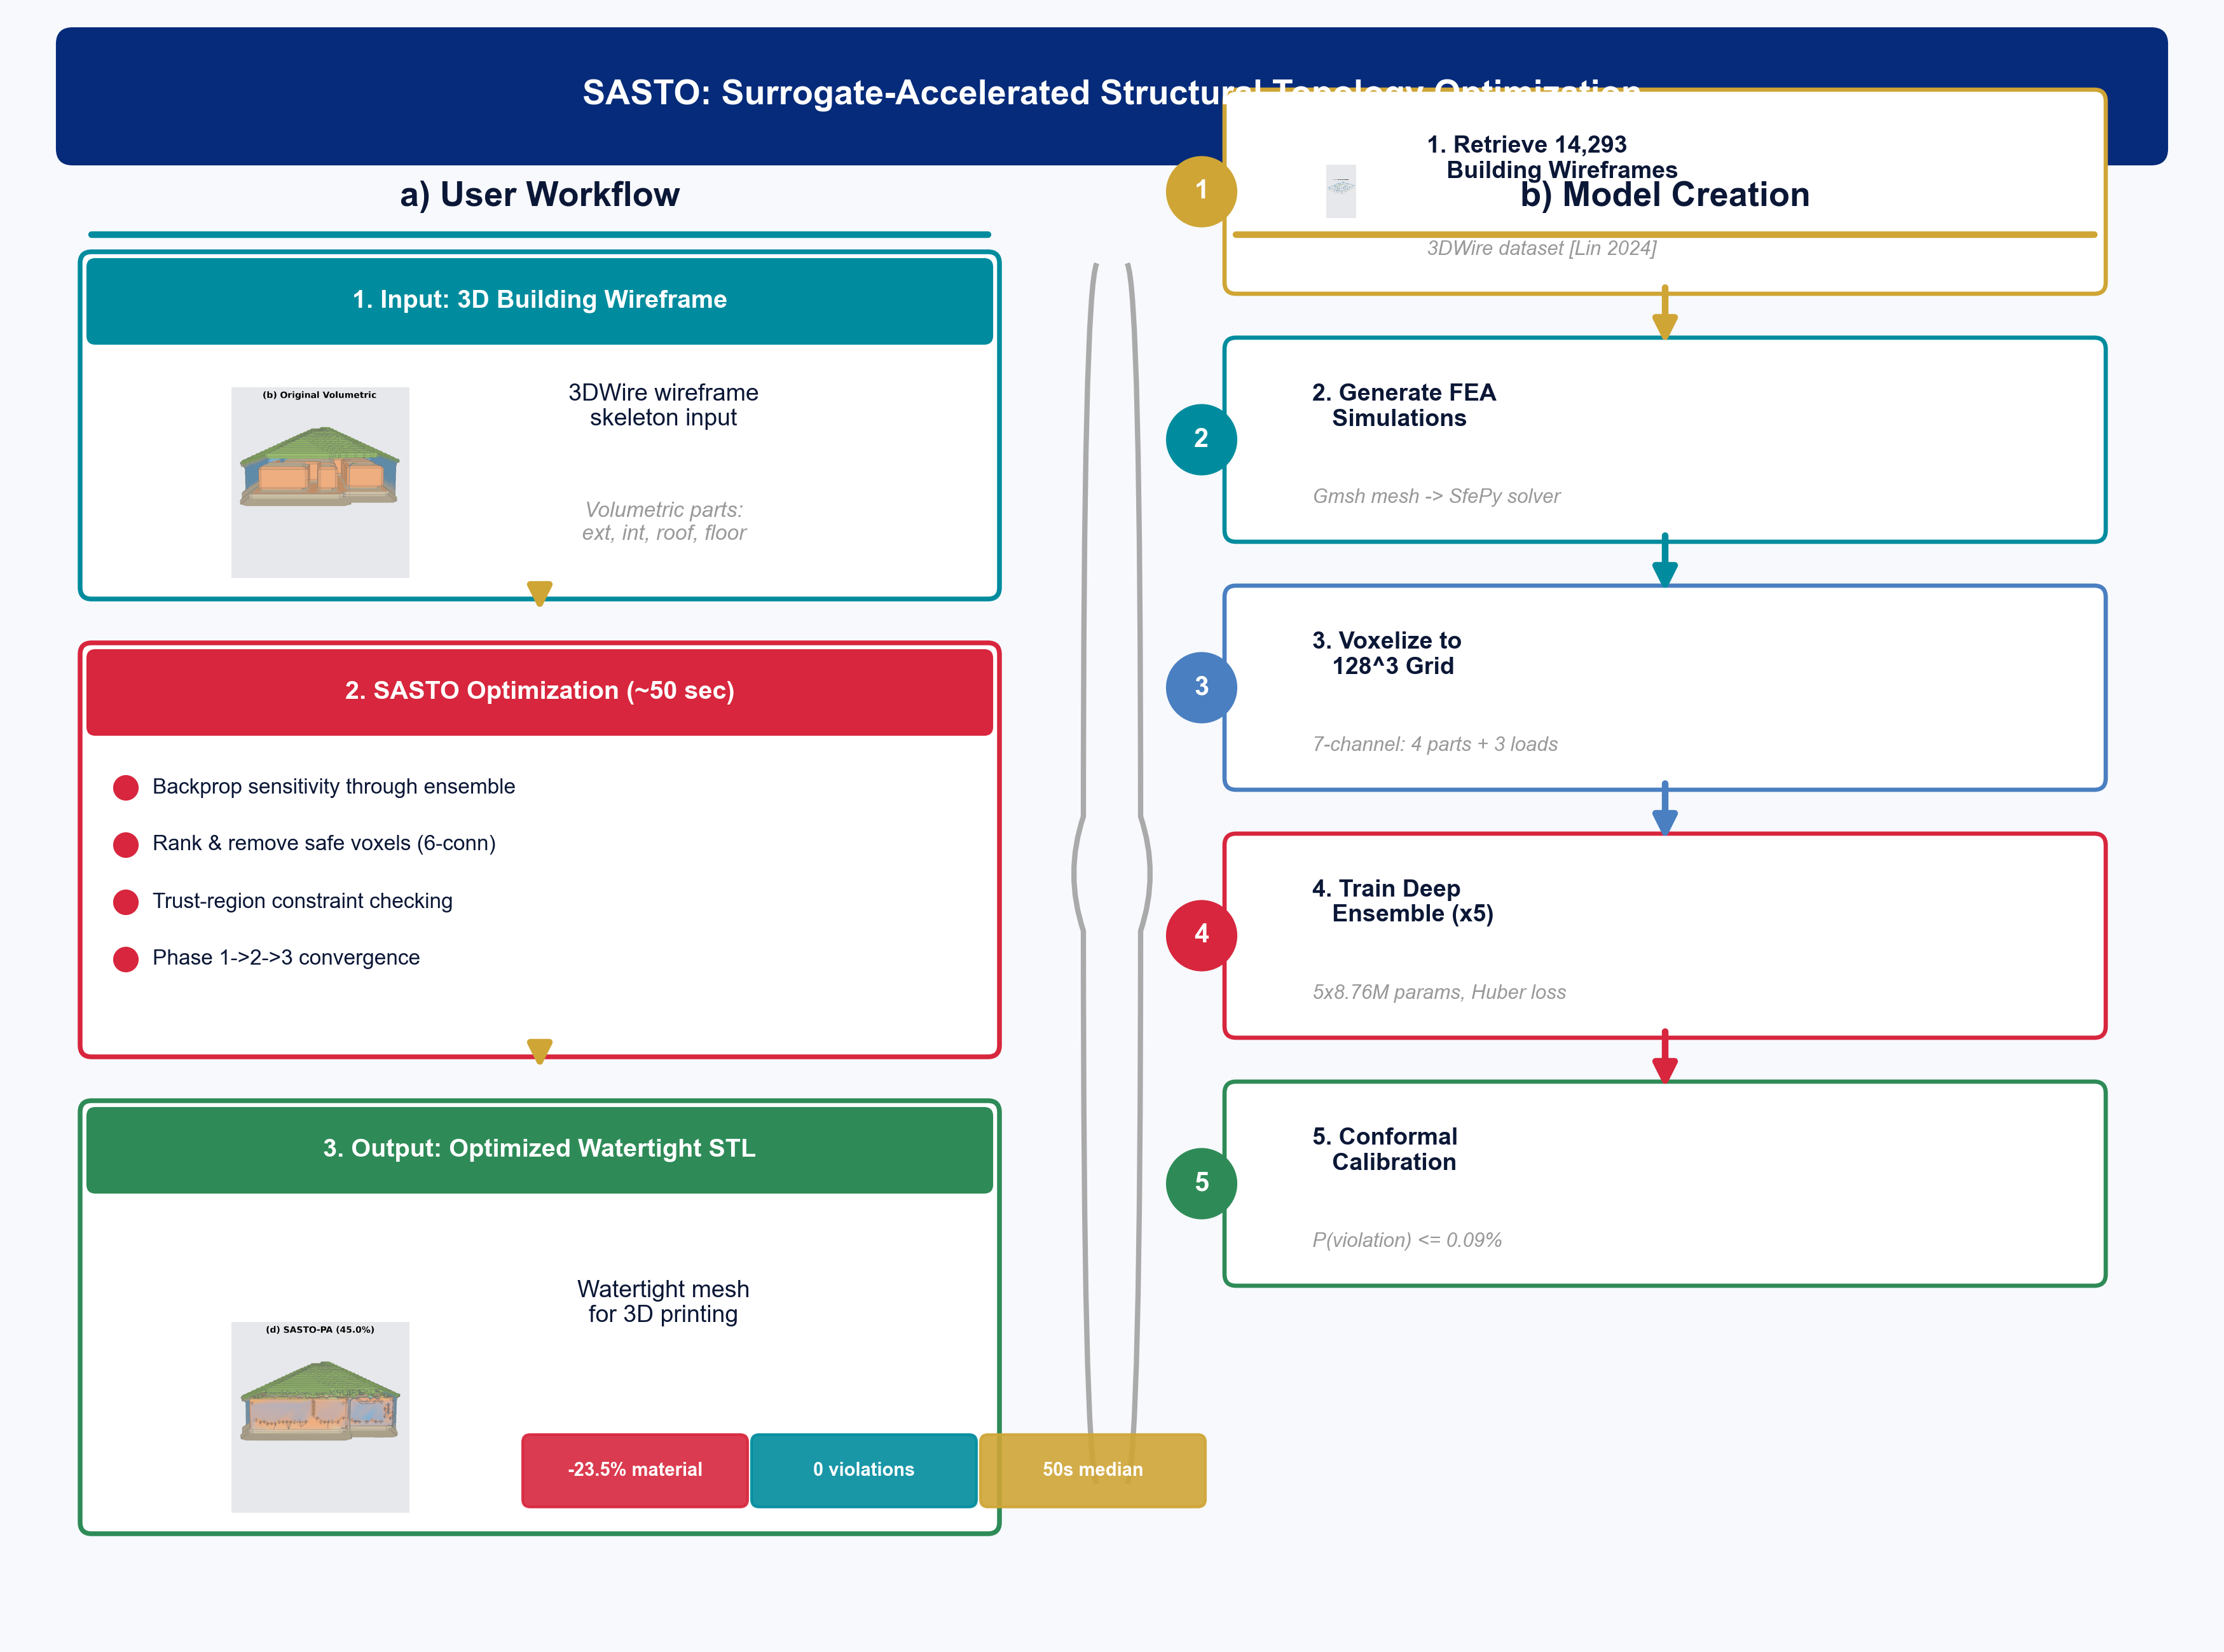
\includegraphics[width=10cm, height=6cm, keepaspectratio]{fig01_visual_abstract_pipeline.png}\\[2pt]
                SASTO Optimization}
                \vspace{0.2cm}
            \end{minipage}
        }
    };
    
    % Center text
    \node[anchor=north, inner sep=0] at ([yshift=-1.0cm]current page.north) {
        \begin{minipage}{74cm}
            \centering
            {\fontsize{62}{72}\selectfont\bfseries\color{white}
            SURROGATE-ACCELERATED STRUCTURAL OPTIMIZATION}\\[8pt]
            {\fontsize{32}{38}\selectfont\bfseries\itshape\color{white}
            Additive Manufacturing: Harnessing FEA to Optimize Material Efficiency}\\[8pt]
            {\fontsize{26}{32}\selectfont\bfseries\color{white}
            Eric Hou}
        \end{minipage}
    };
    
    % Right credit block
    \node[anchor=north east, inner sep=0, text width=15cm] at ([xshift=-1cm, yshift=-0.5cm]current page.north east) {
        \raggedleft
        {\fontsize{14}{17}\selectfont\bfseries\color{white}Credit Line of Origin}\\[2pt]
        {\fontsize{13}{16}\selectfont\color{white}\itshape References \& data in references below.}\\[2pt]
        {\fontsize{13}{16}\selectfont\color{white}
        Images denoted with asterisk are\\
        public domain or adapted sources.}\\[2pt]
        {\fontsize{13}{16}\selectfont\color{white}
        All other graphics, tables, and images\\
        have been created by Eric Hou, 2026\\
        unless otherwise attributed.}
    };
\end{tikzpicture}

\vspace{8.5cm} % Space below title band

% ════════════════════════════════════════════════════════════════
% THREE-COLUMN LAYOUT
% ════════════════════════════════════════════════════════════════
\begin{columns}[T]

% ══════════════════════════════════════════════════════════════
% LEFT PANEL (12 inches = 30.48cm)
% ══════════════════════════════════════════════════════════════
\begin{column}{0.25\textwidth}

% ── L1: VISUAL ABSTRACT ──────────────────────────────────────
\begin{sectionbox}{Visual Abstract}
\bodytext
\centering
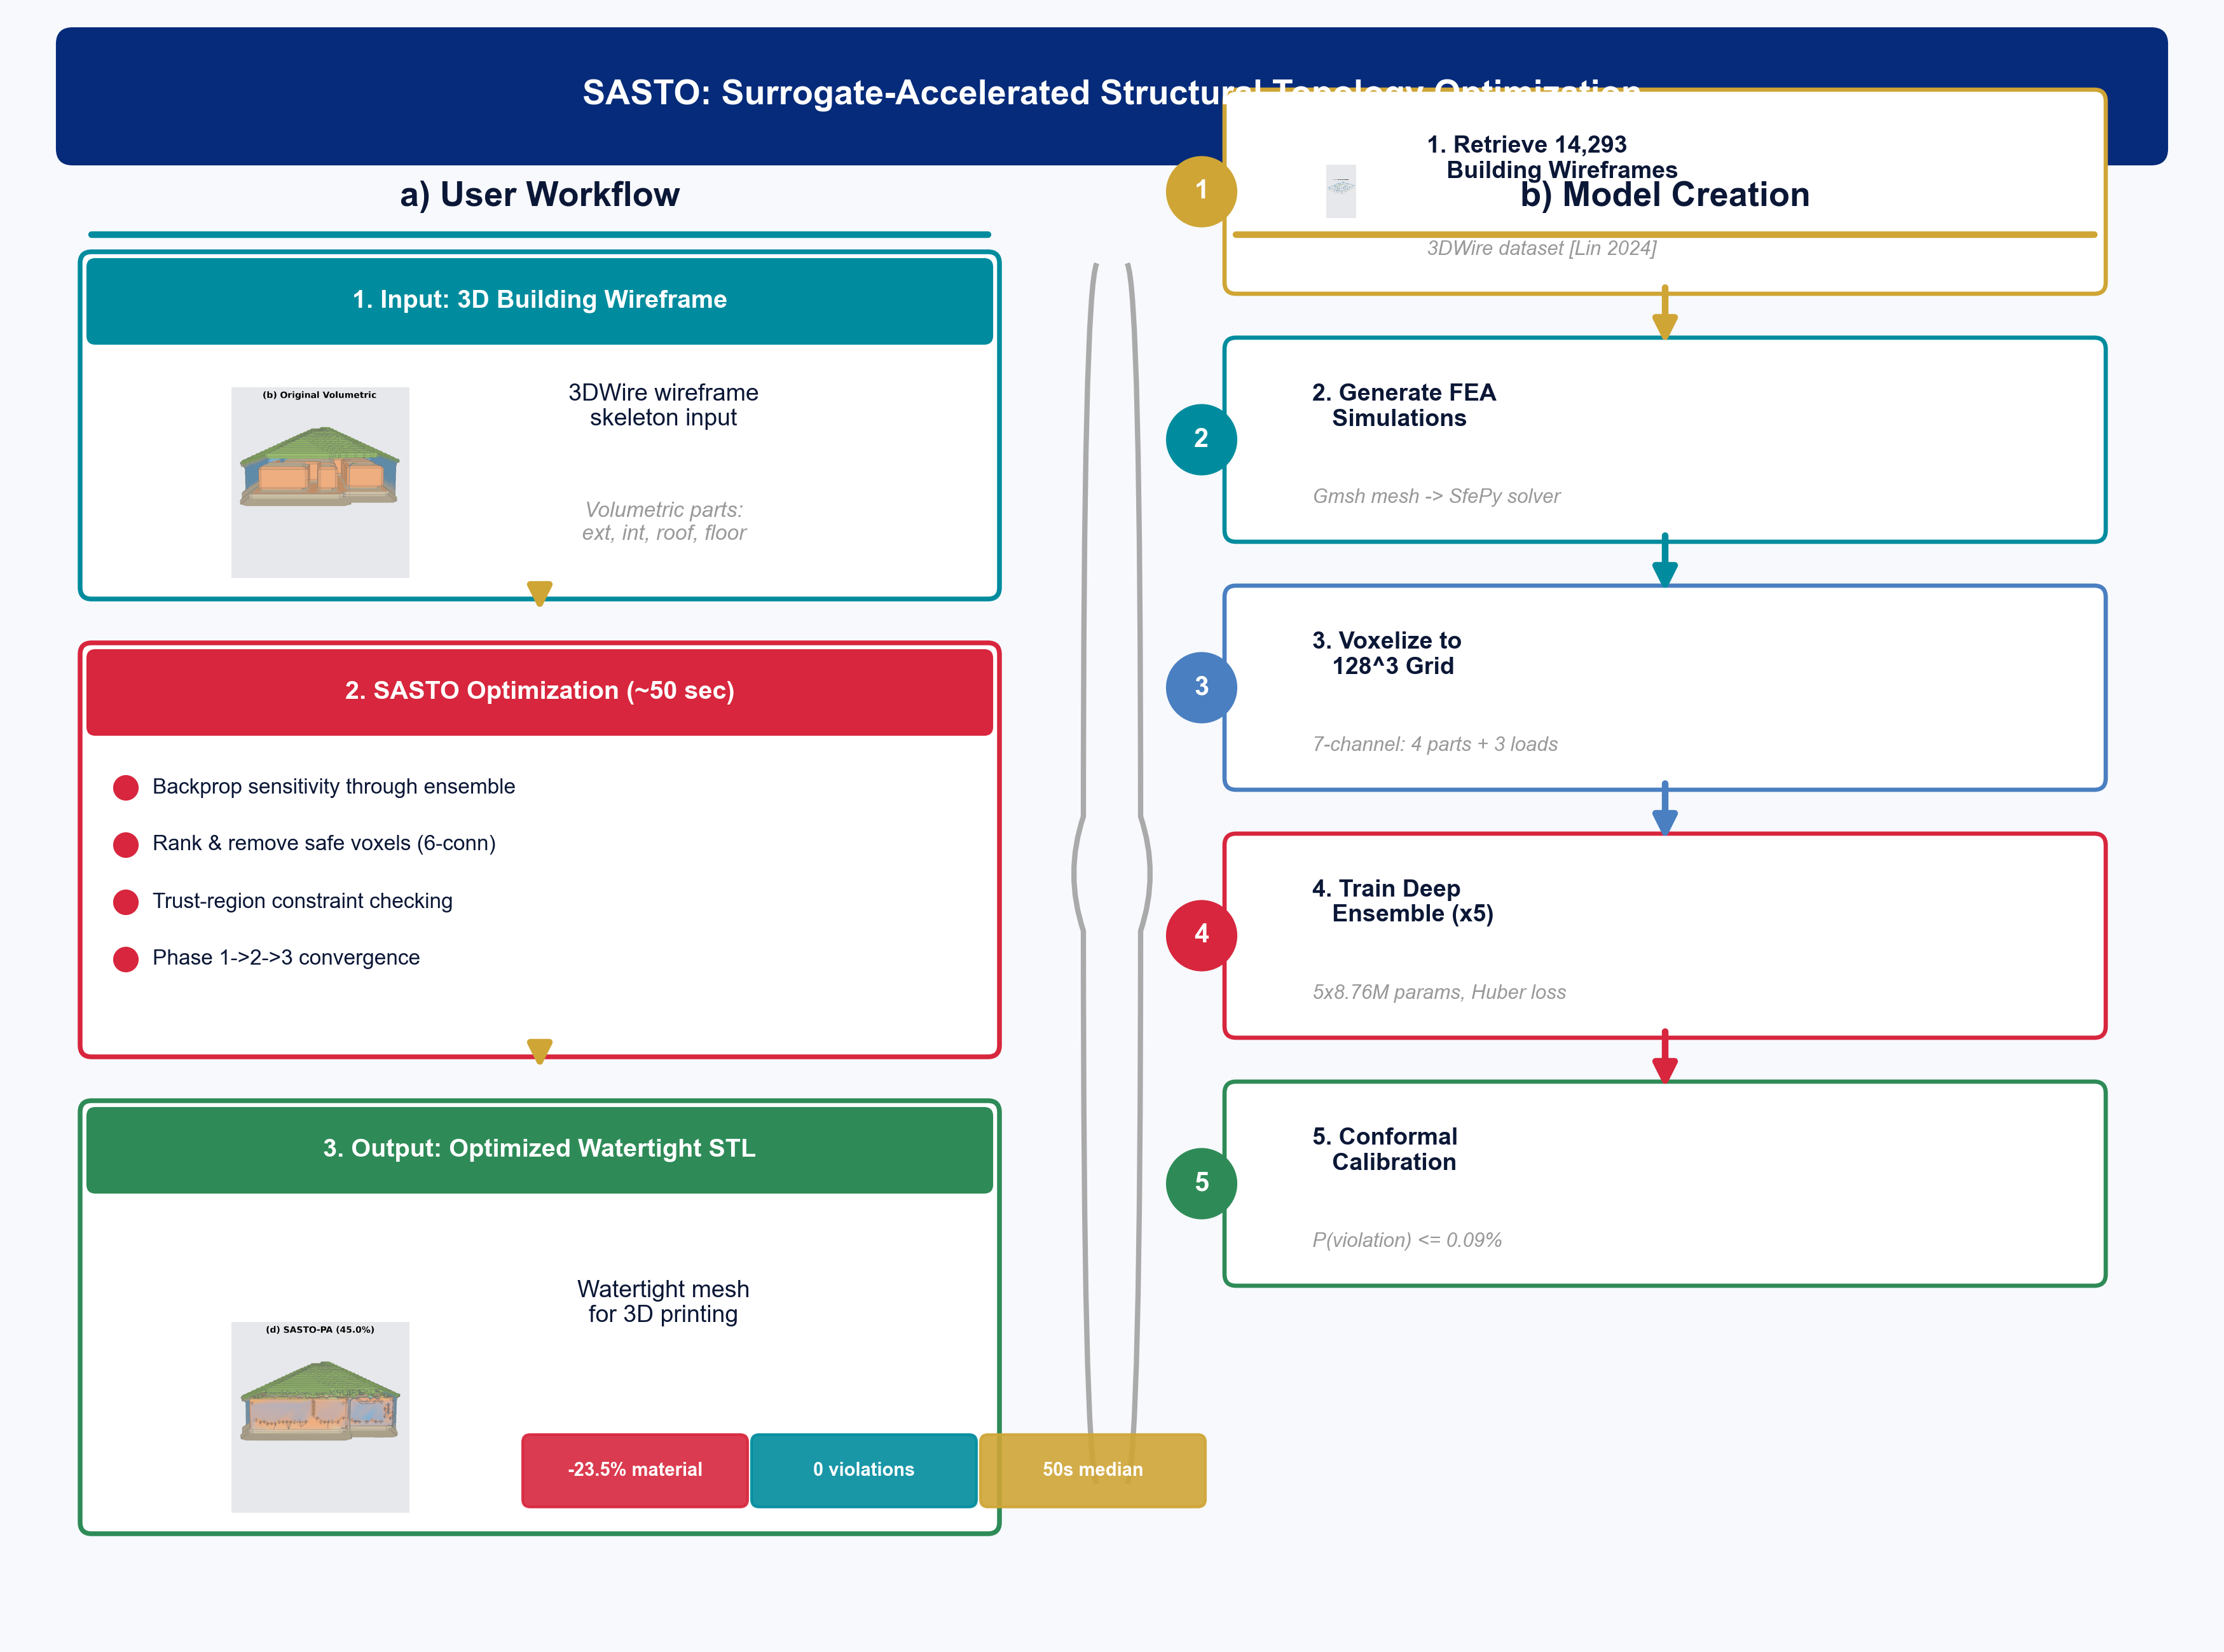
\includegraphics[width=\linewidth]{fig01_visual_abstract_pipeline.png}\\[2pt]
{\captiontext Fig.~1. SASTO pipeline: offline training (Steps 1--4) and online optimization (Steps 4--6). A building wireframe becomes a watertight optimized STL in $\sim$50 seconds.}
\end{sectionbox}

\vspace{4pt}

% ── L2: INTRODUCTION ─────────────────────────────────────────
\begin{sectionbox}{Introduction}
\bodytext

\subheader{Concrete \& Construction}
Concrete production accounts for $\sim$8\% of global CO\textsubscript{2} emissions~[IEA 2021]. Conventional construction uses uniform-thickness walls determined by formwork constraints, not structural need---a substantial source of wasted material.

\subheader{Additive Manufacturing Opportunity}
Large-scale 3D concrete printing (ICON, COBOD, Apis Cor) can realize arbitrary wall profiles at no marginal tooling cost, enabling topology-optimized structures that place material only where structurally required.

\subheader{The Computational Bottleneck}
Classical topology optimization (SIMP) requires hundreds of FEA solves---each taking minutes to hours at building scale---making it computationally intractable. Voxel-based methods produce disconnected fragments incompatible with 3D printing.

\vspace{4pt}
\centering
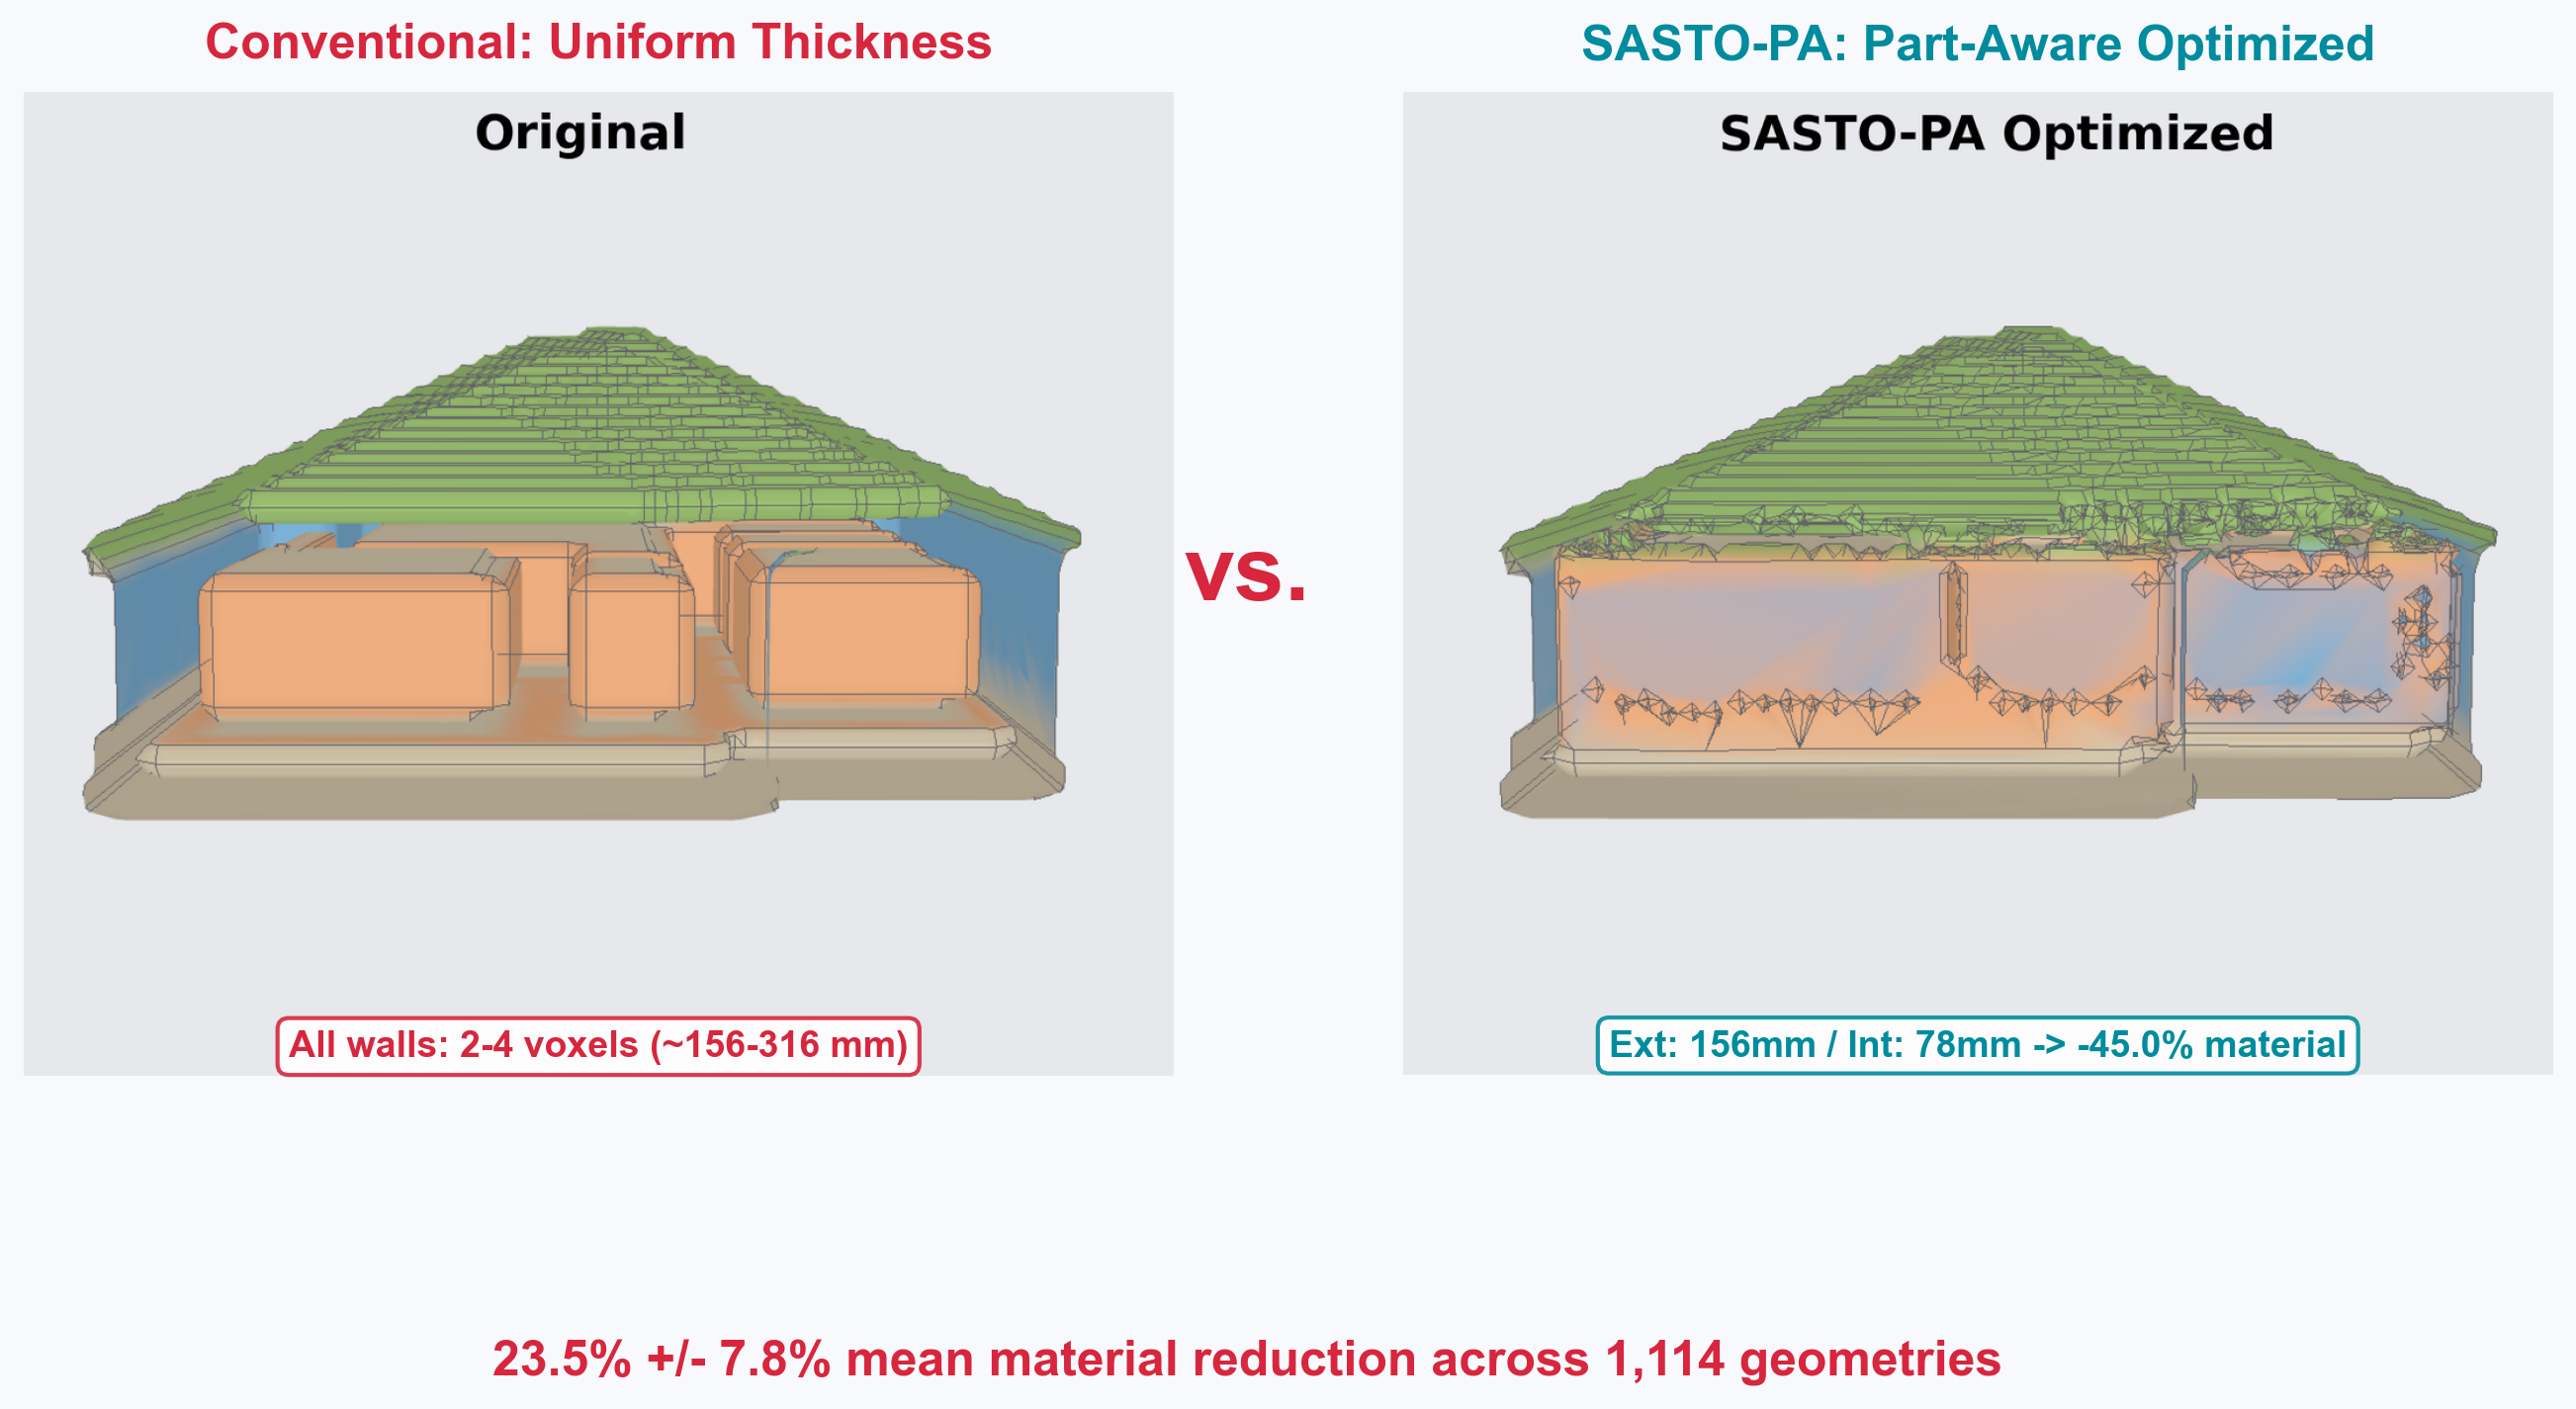
\includegraphics[width=\linewidth]{fig02_uniform_vs_optimized.png}\\[2pt]
{\captiontext Fig.~2. Uniform-wall construction vs.\ SASTO part-aware optimization.}
\end{sectionbox}

\vspace{4pt}

% ── L3: RESEARCH OBJECTIVES ──────────────────────────────────
\begin{sectionbox}{Research Objectives}
\bodytext

\begin{enumerate}[leftmargin=*, itemsep=3pt, label={\color{accentteal}\bfseries\arabic*.}]
    \item \textbf{\color{accentteal}SPEED} --- Deep ensemble surrogate $\to$ 23--92$\times$ speedup over SIMP
    \item \textbf{\color{accentteal}PRINTABILITY} --- 6-connectivity criterion $\to$ single-component watertight STL
    \item \textbf{\color{accentgold}EFFICIENCY} --- Part-aware min thickness $\to$ 10.7pp more reduction than uniform
    \item \textbf{\color{accentred}SAFETY} --- Uncertainty-aware constraints $\to$ 0/1,114 violations, $P \le 0.09\%$
\end{enumerate}

\vspace{4pt}
\centering
\begin{tikzpicture}[
    box/.style={rectangle, rounded corners=4pt, minimum width=5.5cm, minimum height=1.2cm, 
        fill=accentteal, text=white, font=\fontsize{11}{13}\selectfont\bfseries, align=center},
    arr/.style={-{Stealth[length=6pt]}, white, line width=2pt}
]
\node[box] (d1) {1. Data Generation};
\node[box, right=0.3cm of d1] (d2) {2. Surrogate Training};
\node[box, right=0.3cm of d2] (d3) {3. SASTO Optimize};
\node[box, right=0.3cm of d3] (d4) {4. Validate};
\draw[arr] (d1) -- (d2);
\draw[arr] (d2) -- (d3);
\draw[arr] (d3) -- (d4);
\end{tikzpicture}
\end{sectionbox}

\vspace{4pt}

% ── L4: ENGINEERING DESIGN CRITERIA ──────────────────────────
\begin{sectionbox}{Engineering Design Criteria}
\bodytext
\centering
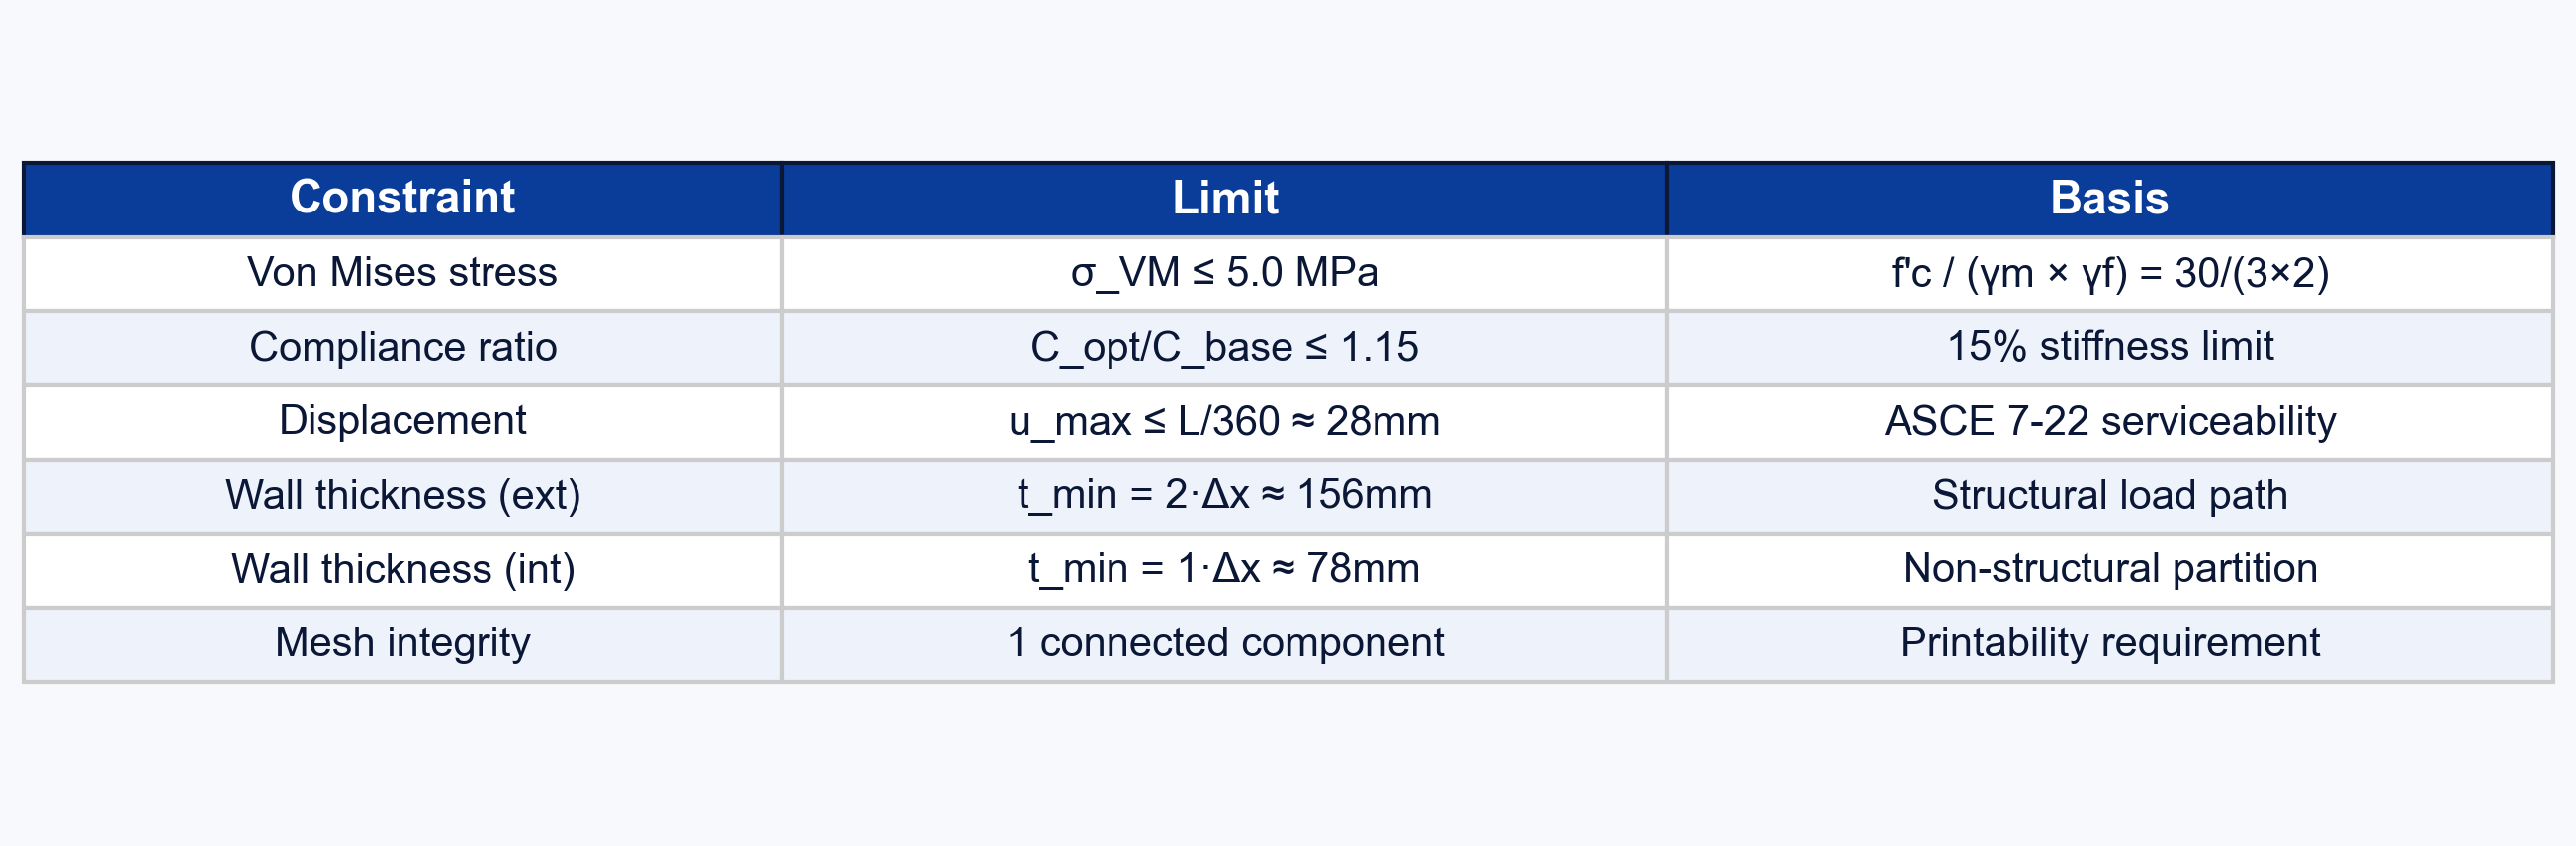
\includegraphics[width=\linewidth]{fig18_design_criteria_table.png}

\vspace{4pt}
\begin{eqbox}
\centering
$\sigma_{\mathrm{VM,allow}} = \dfrac{f'_c}{\gamma_m \times \gamma_f} = \dfrac{30}{3.0 \times 2.0} = 5.0~\mathrm{MPa}$\\[4pt]
{\small Conservative ensemble bound: $\hat{\sigma}^+_\mathrm{VM} = \mu_\sigma + k \cdot \sigma_\sigma$, \quad $k = 1.0$}
\end{eqbox}
\end{sectionbox}

\vspace{4pt}

% ── L5: PROBLEM FRAMING ──────────────────────────────────────
\begin{sectionbox}{Problem Framing}
\bodytext

\subheader{Optimization Objective}
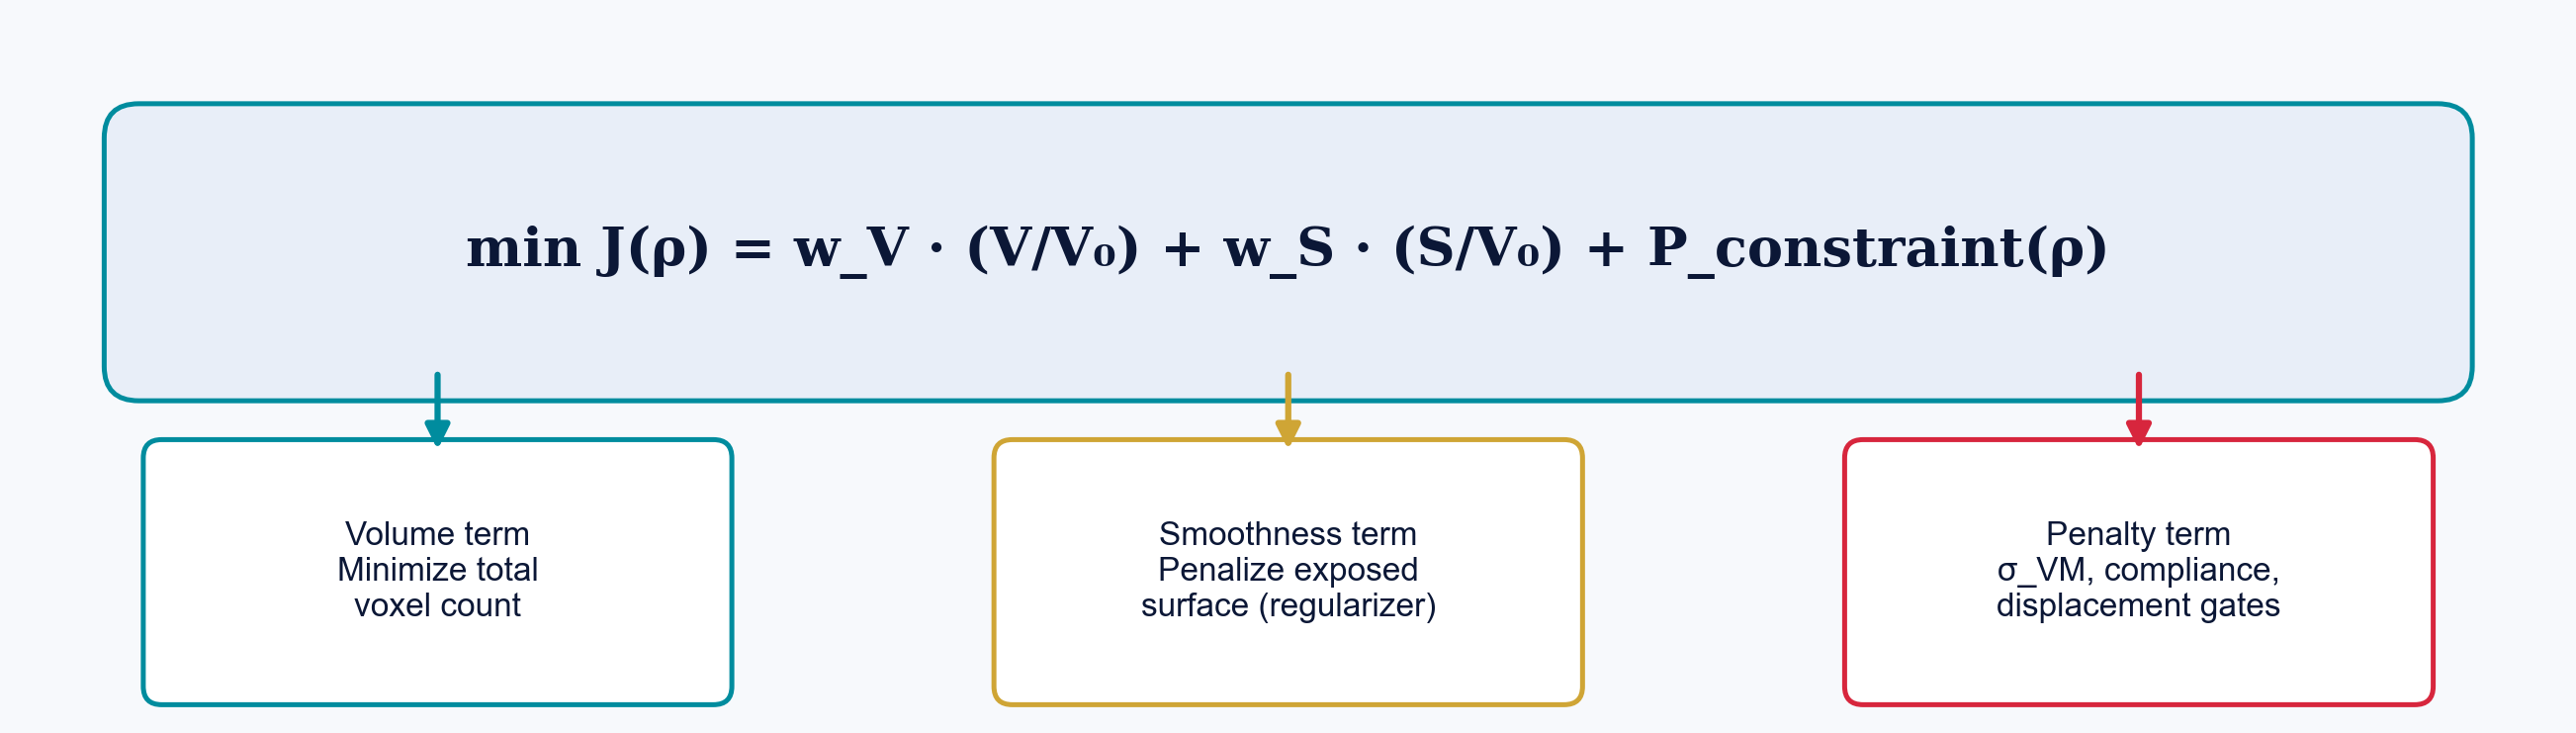
\includegraphics[width=\linewidth]{fig16_optimization_objective.png}

\vspace{4pt}
\subheader{Sensitivity Formula}
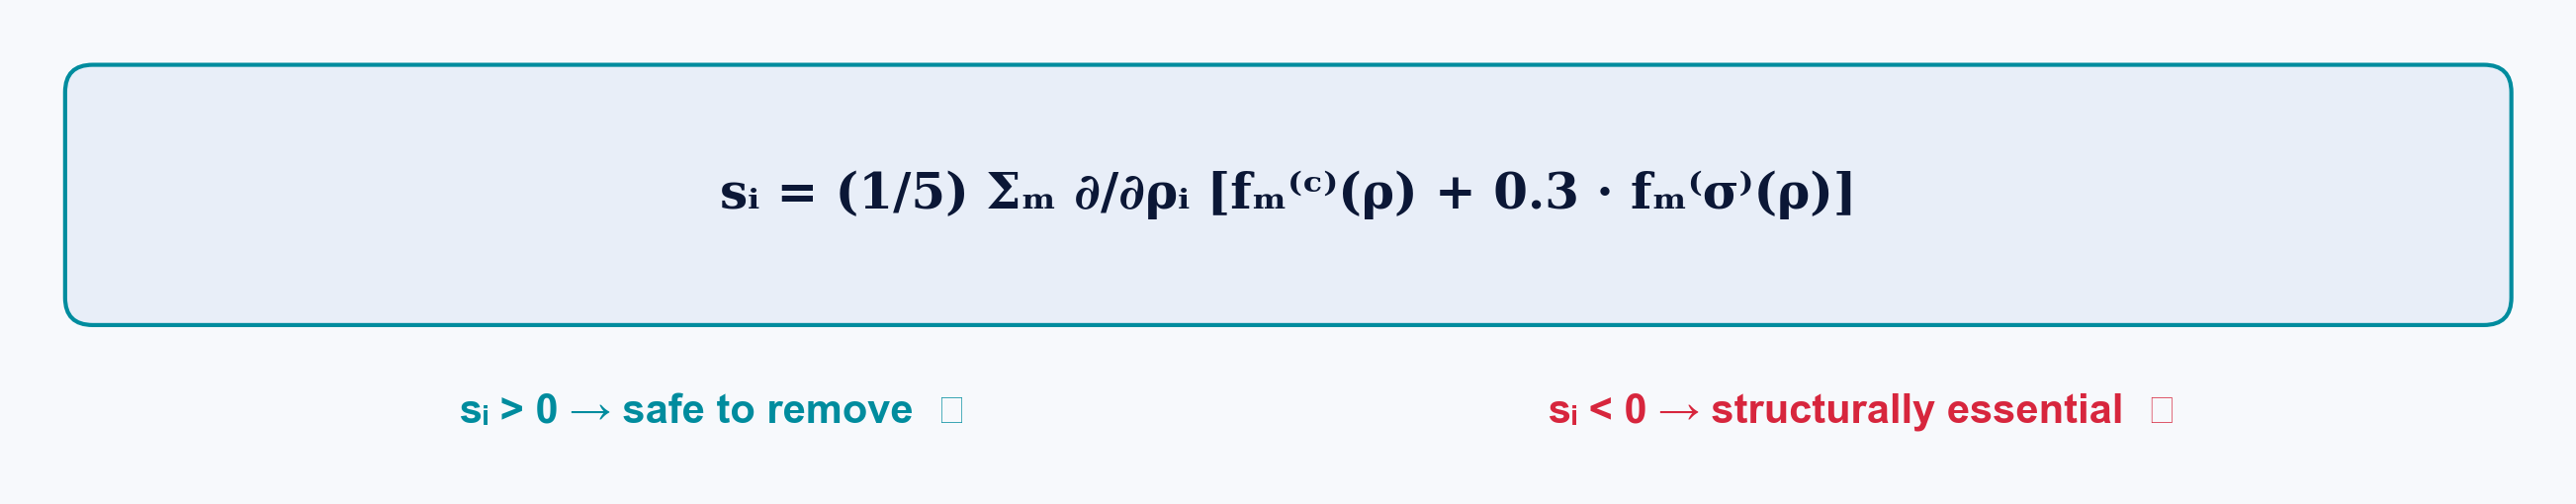
\includegraphics[width=\linewidth]{fig17_sensitivity_formula.png}

\vspace{4pt}
\subheader{Part-Aware Thickness}
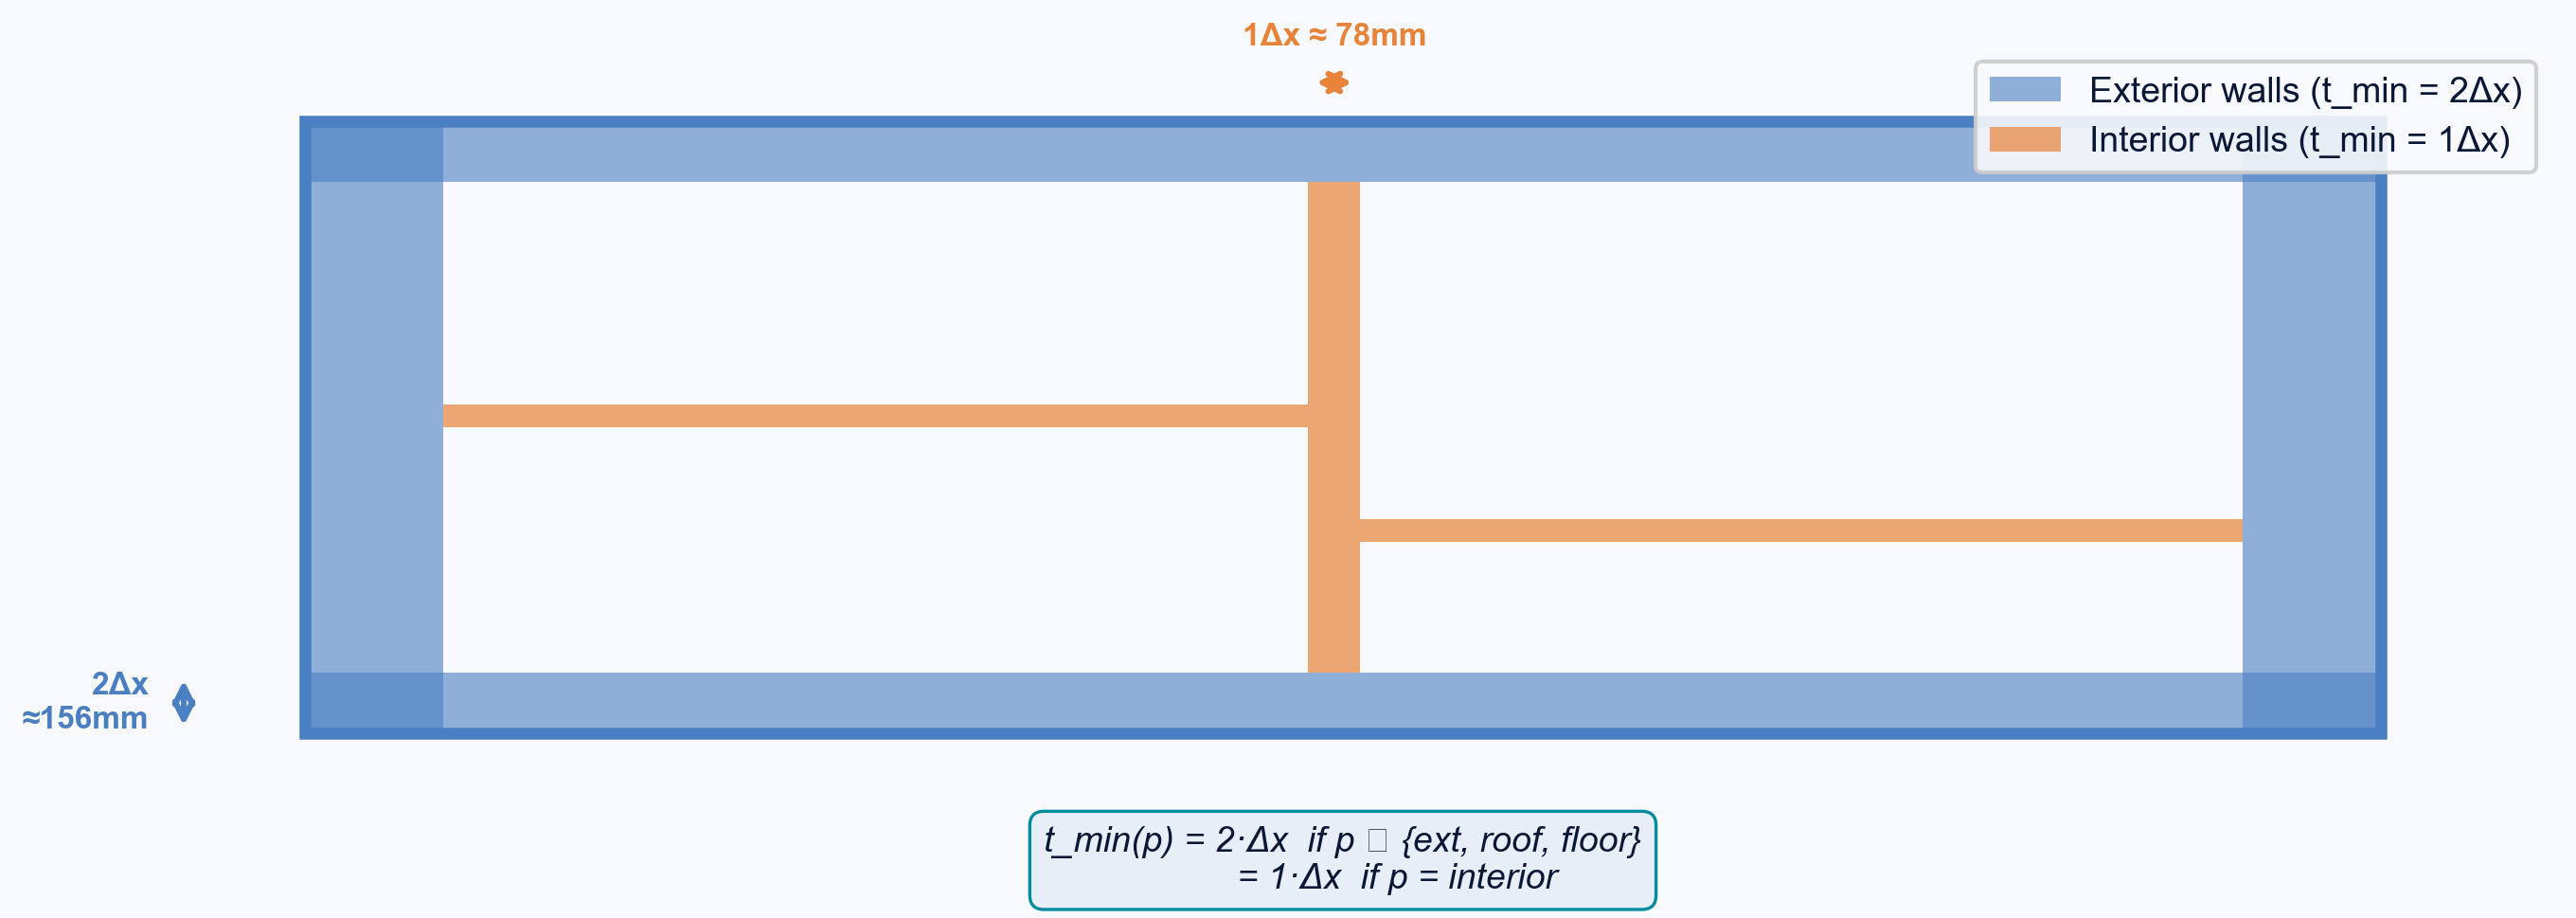
\includegraphics[width=\linewidth]{fig14_part_aware_thickness.png}\\[2pt]
{\captiontext Fig.~5. Part-aware thickness enables 86.8\% interior wall removal in the reference case with no exterior wall degradation.}
\end{sectionbox}

\end{column}

% ══════════════════════════════════════════════════════════════
% CENTER PANEL (24 inches = 60.96cm)
% ══════════════════════════════════════════════════════════════
\begin{column}{0.50\textwidth}

% ── C1: ENGINEERING METHODOLOGY ──────────────────────────────
\begin{sectionbox}{Engineering Methodology}
\bodytext

\begin{columns}[T]
\begin{column}{0.48\textwidth}
\subheader{Dataset Generation Pipeline}
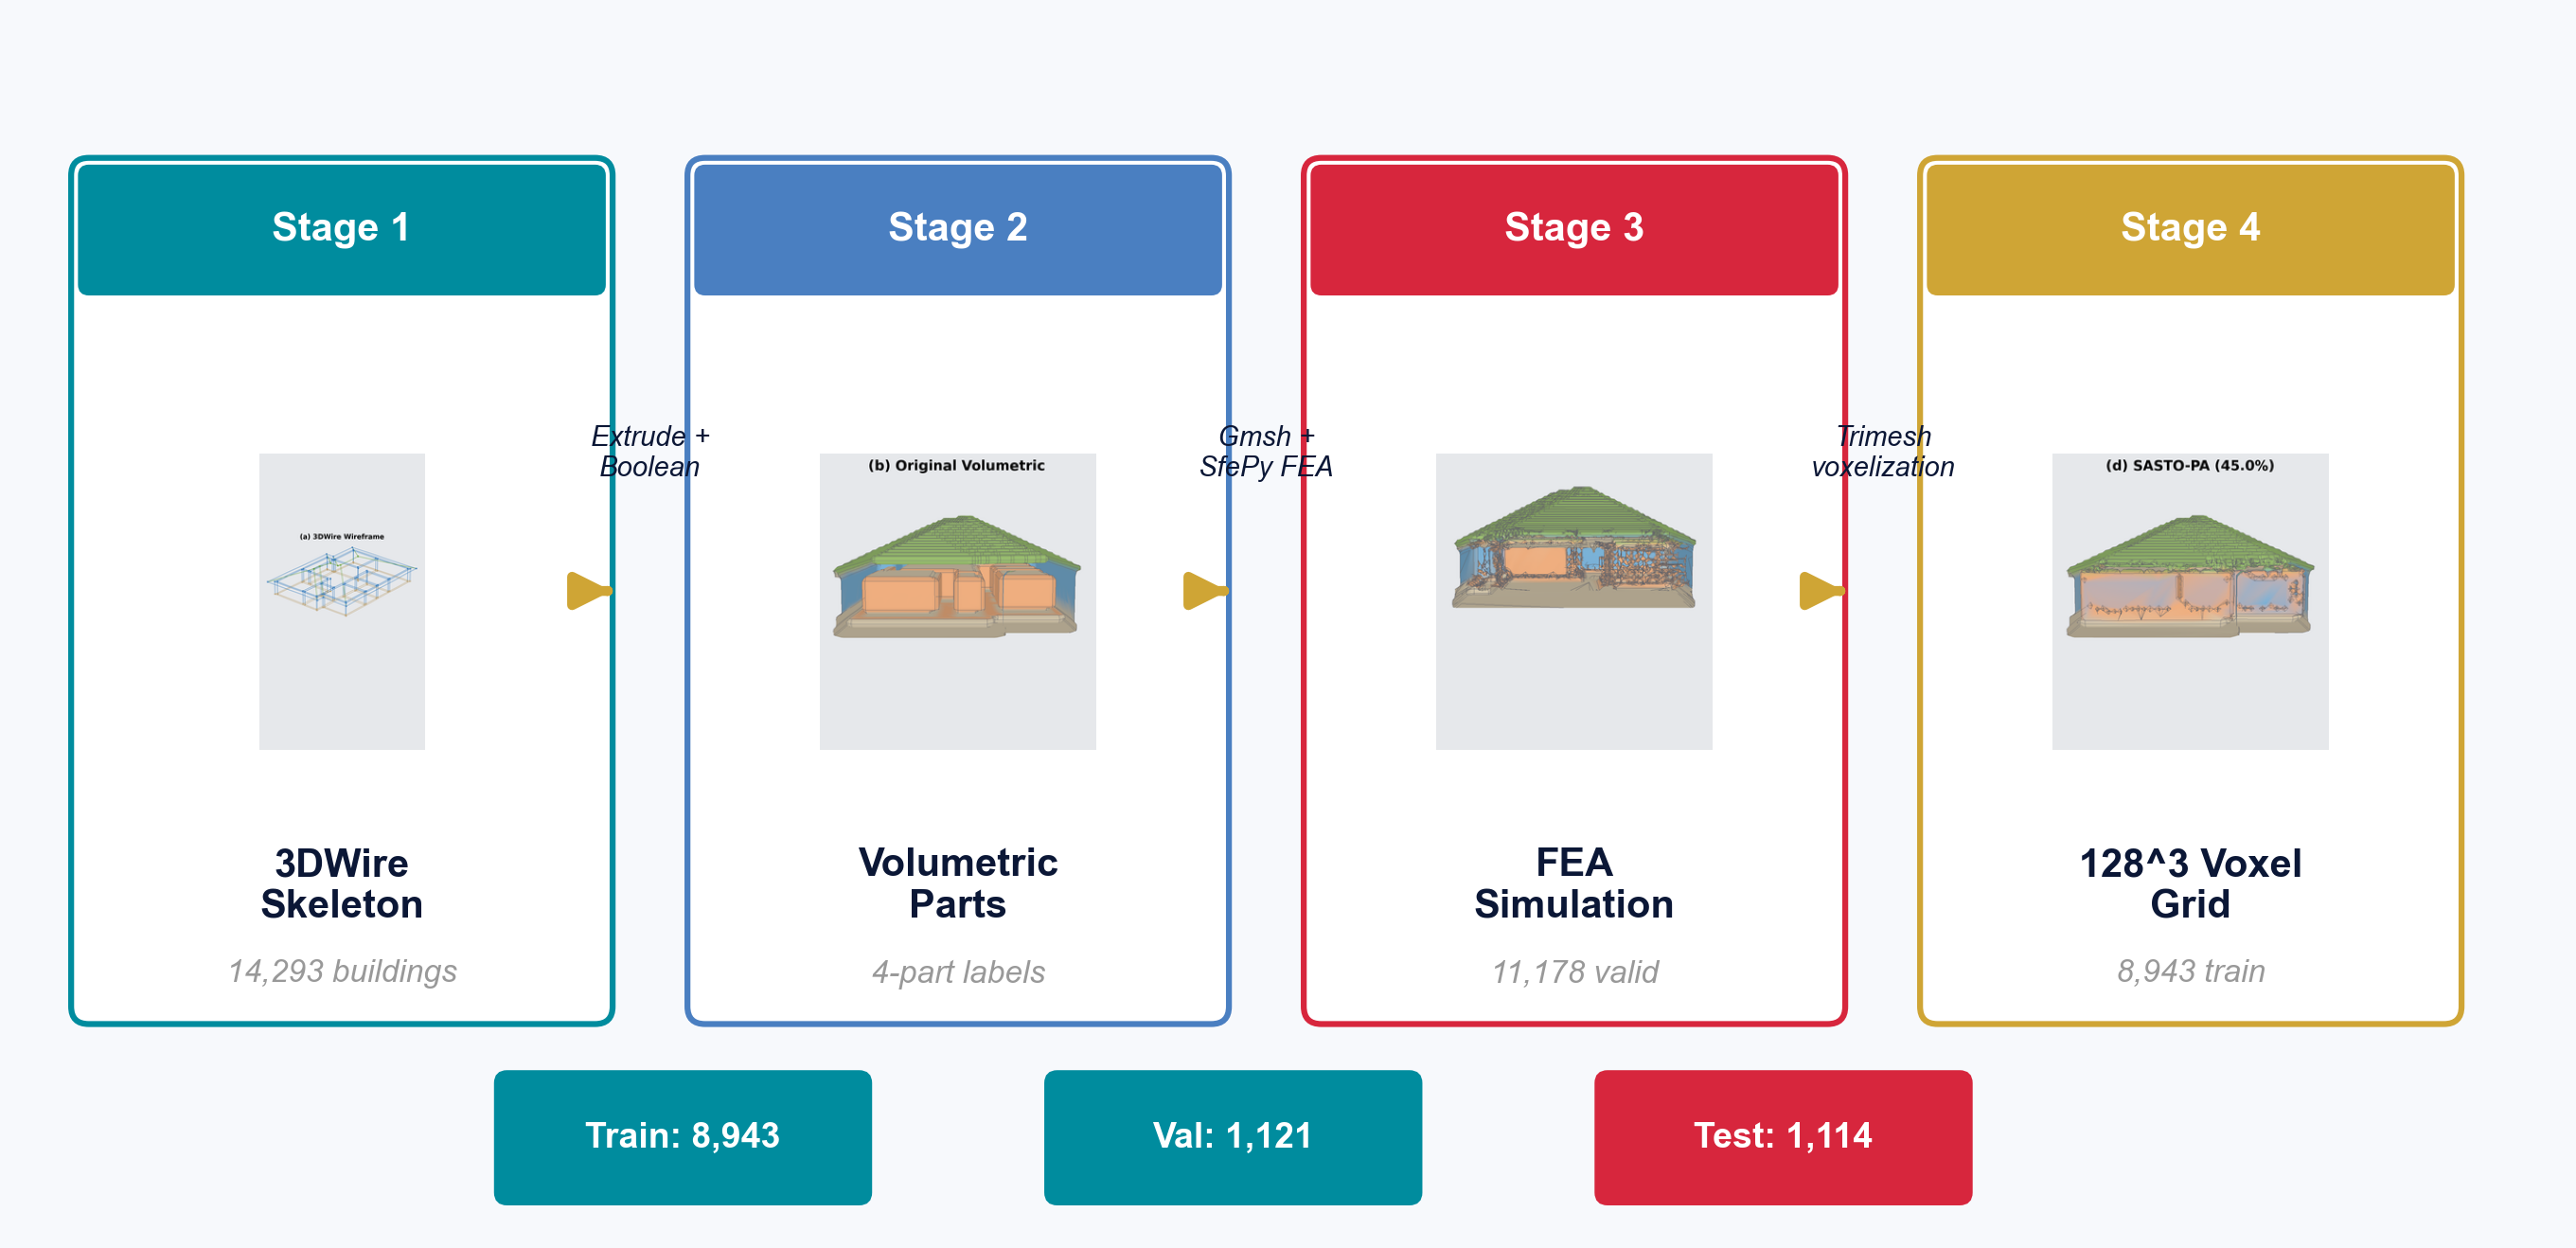
\includegraphics[width=\linewidth]{fig03_dataset_pipeline.png}\\
{\captiontext Fig.~6. Wireframe-to-voxel pipeline. 14,293 wireframes $\to$ 11,178 valid FEA simulations $\to$ 128$^3$ labeled voxel grids.}

\vspace{6pt}
\subheader{Sensitivity-Guided Erosion (SASTO)}
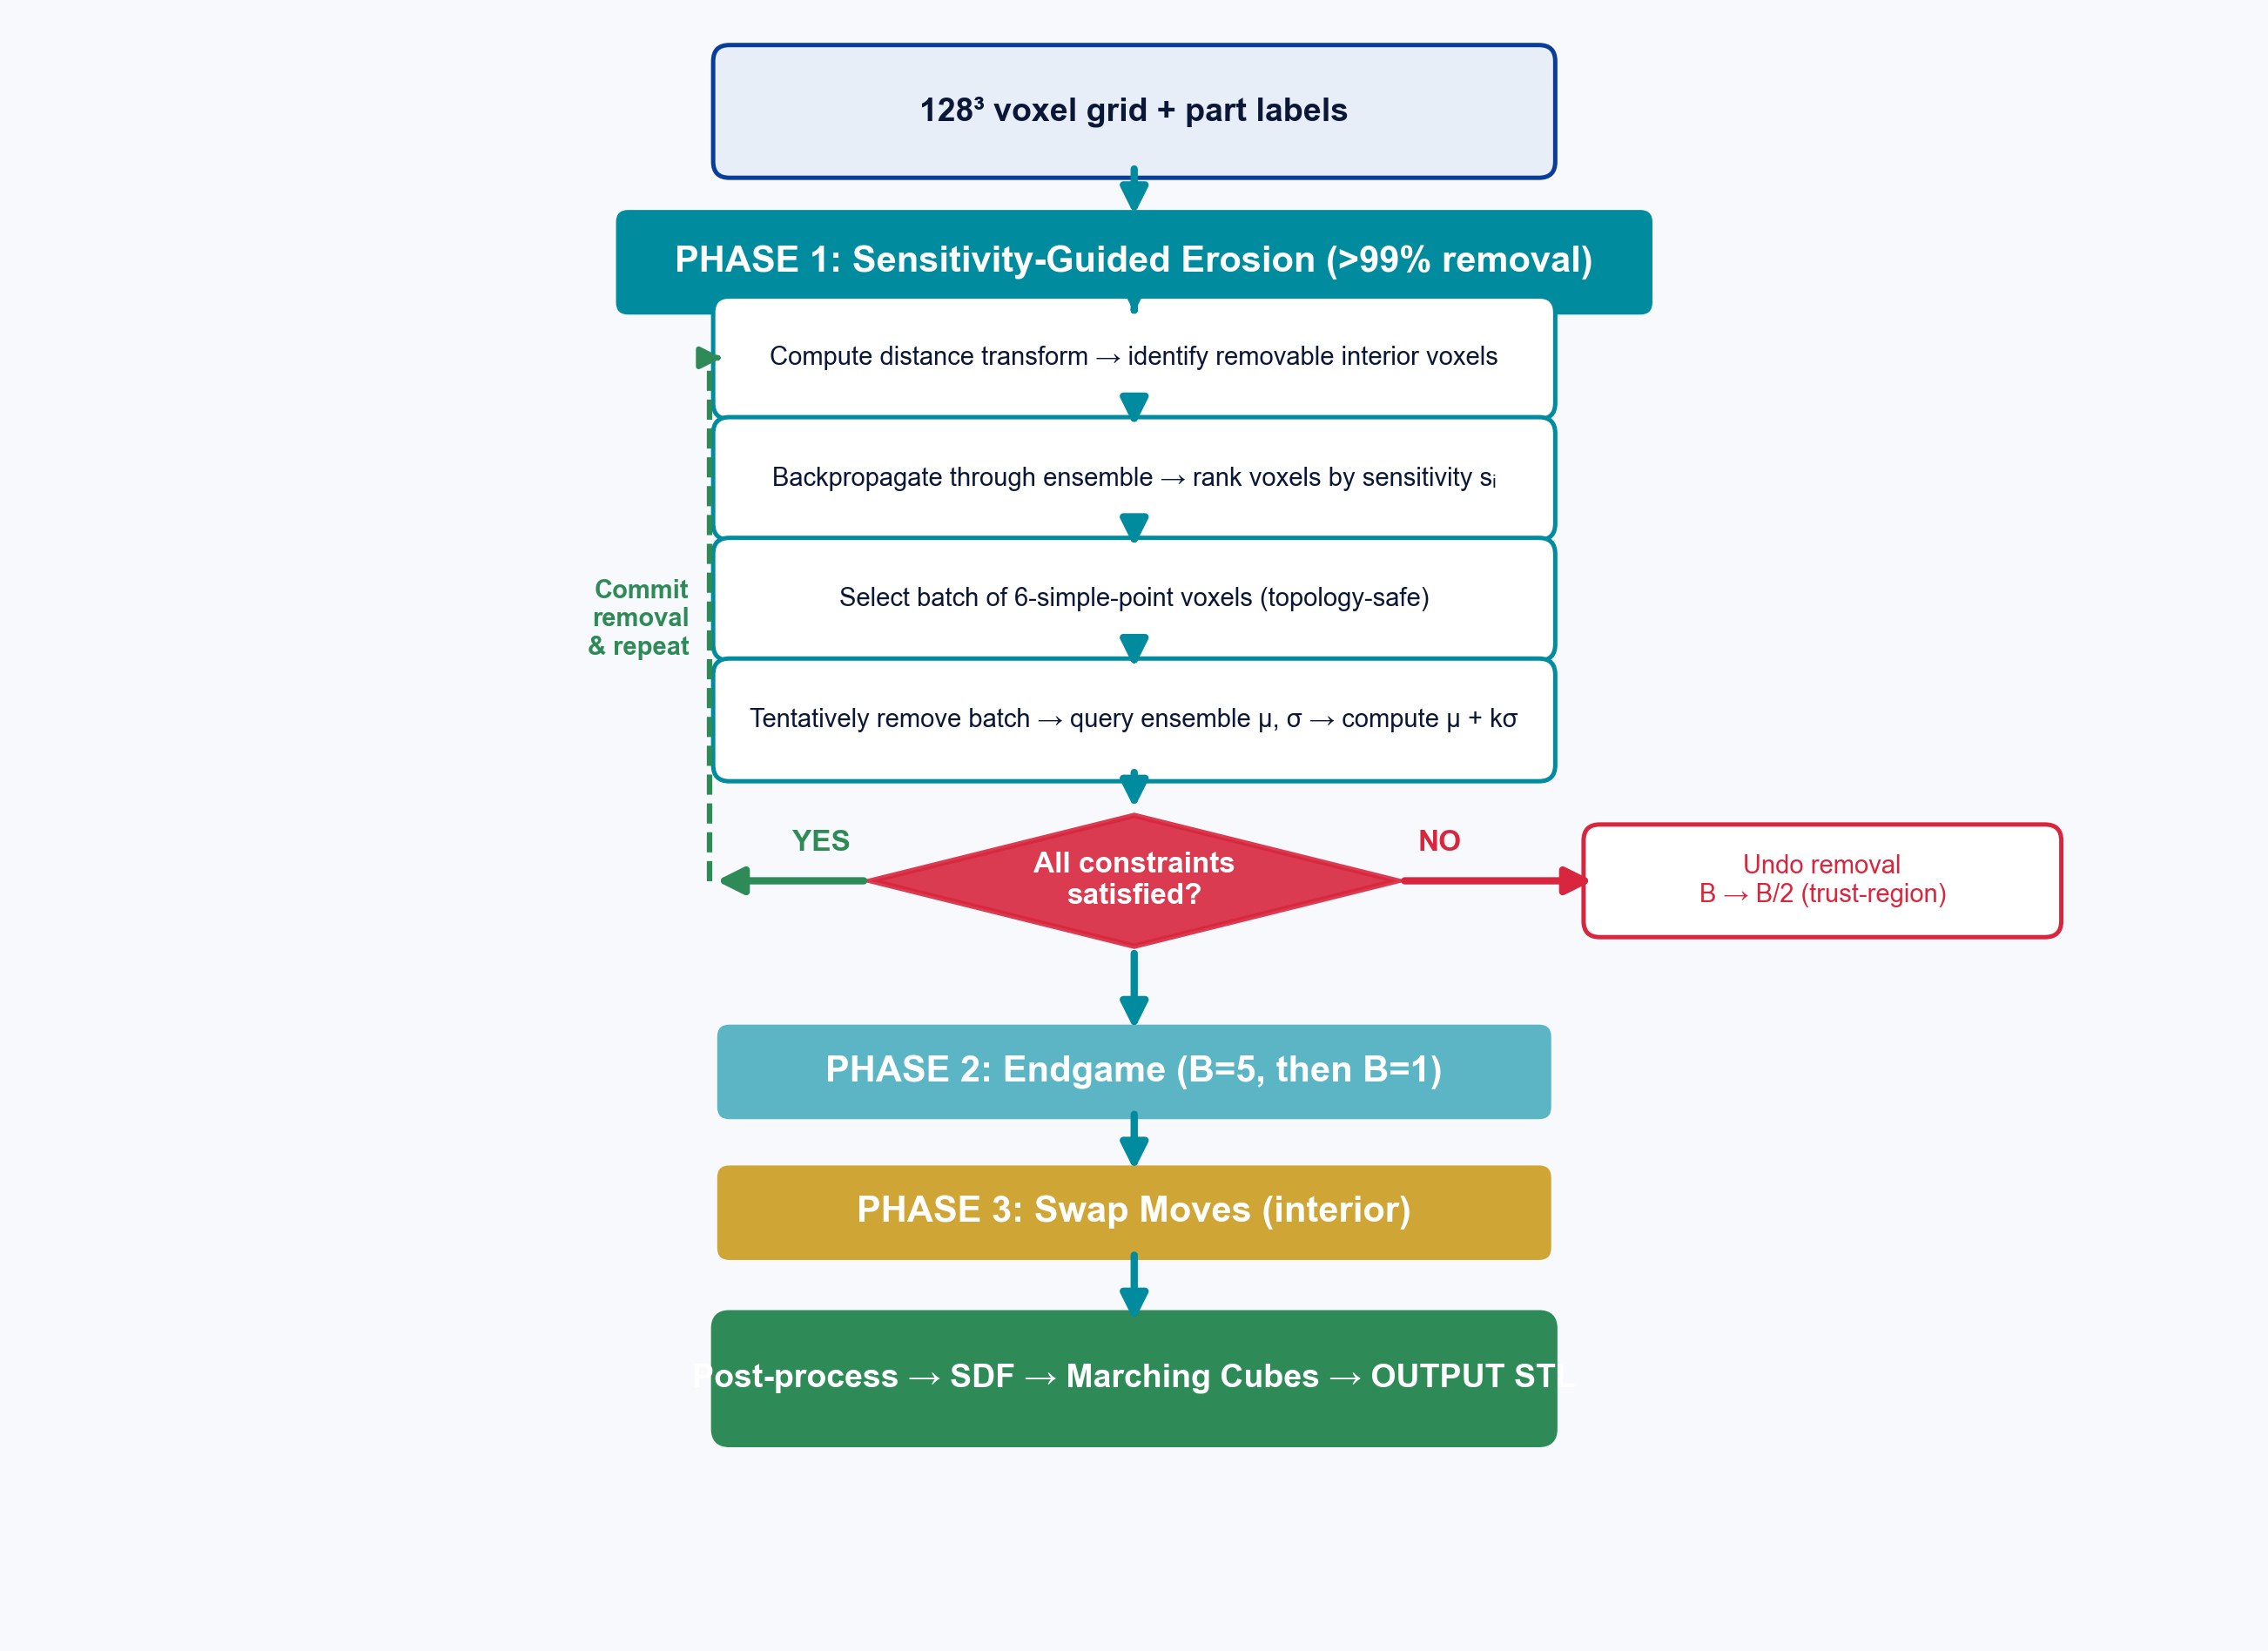
\includegraphics[width=\linewidth]{fig05_sasto_flowchart.png}\\
{\captiontext Fig.~8. SASTO three-phase algorithm. Phase~1 provides {>}99\% of removal via sensitivity ranking + trust-region batch halving.}
\end{column}

\begin{column}{0.48\textwidth}
\subheader{Deep Ensemble Surrogate (5$\times$8.76M params)}
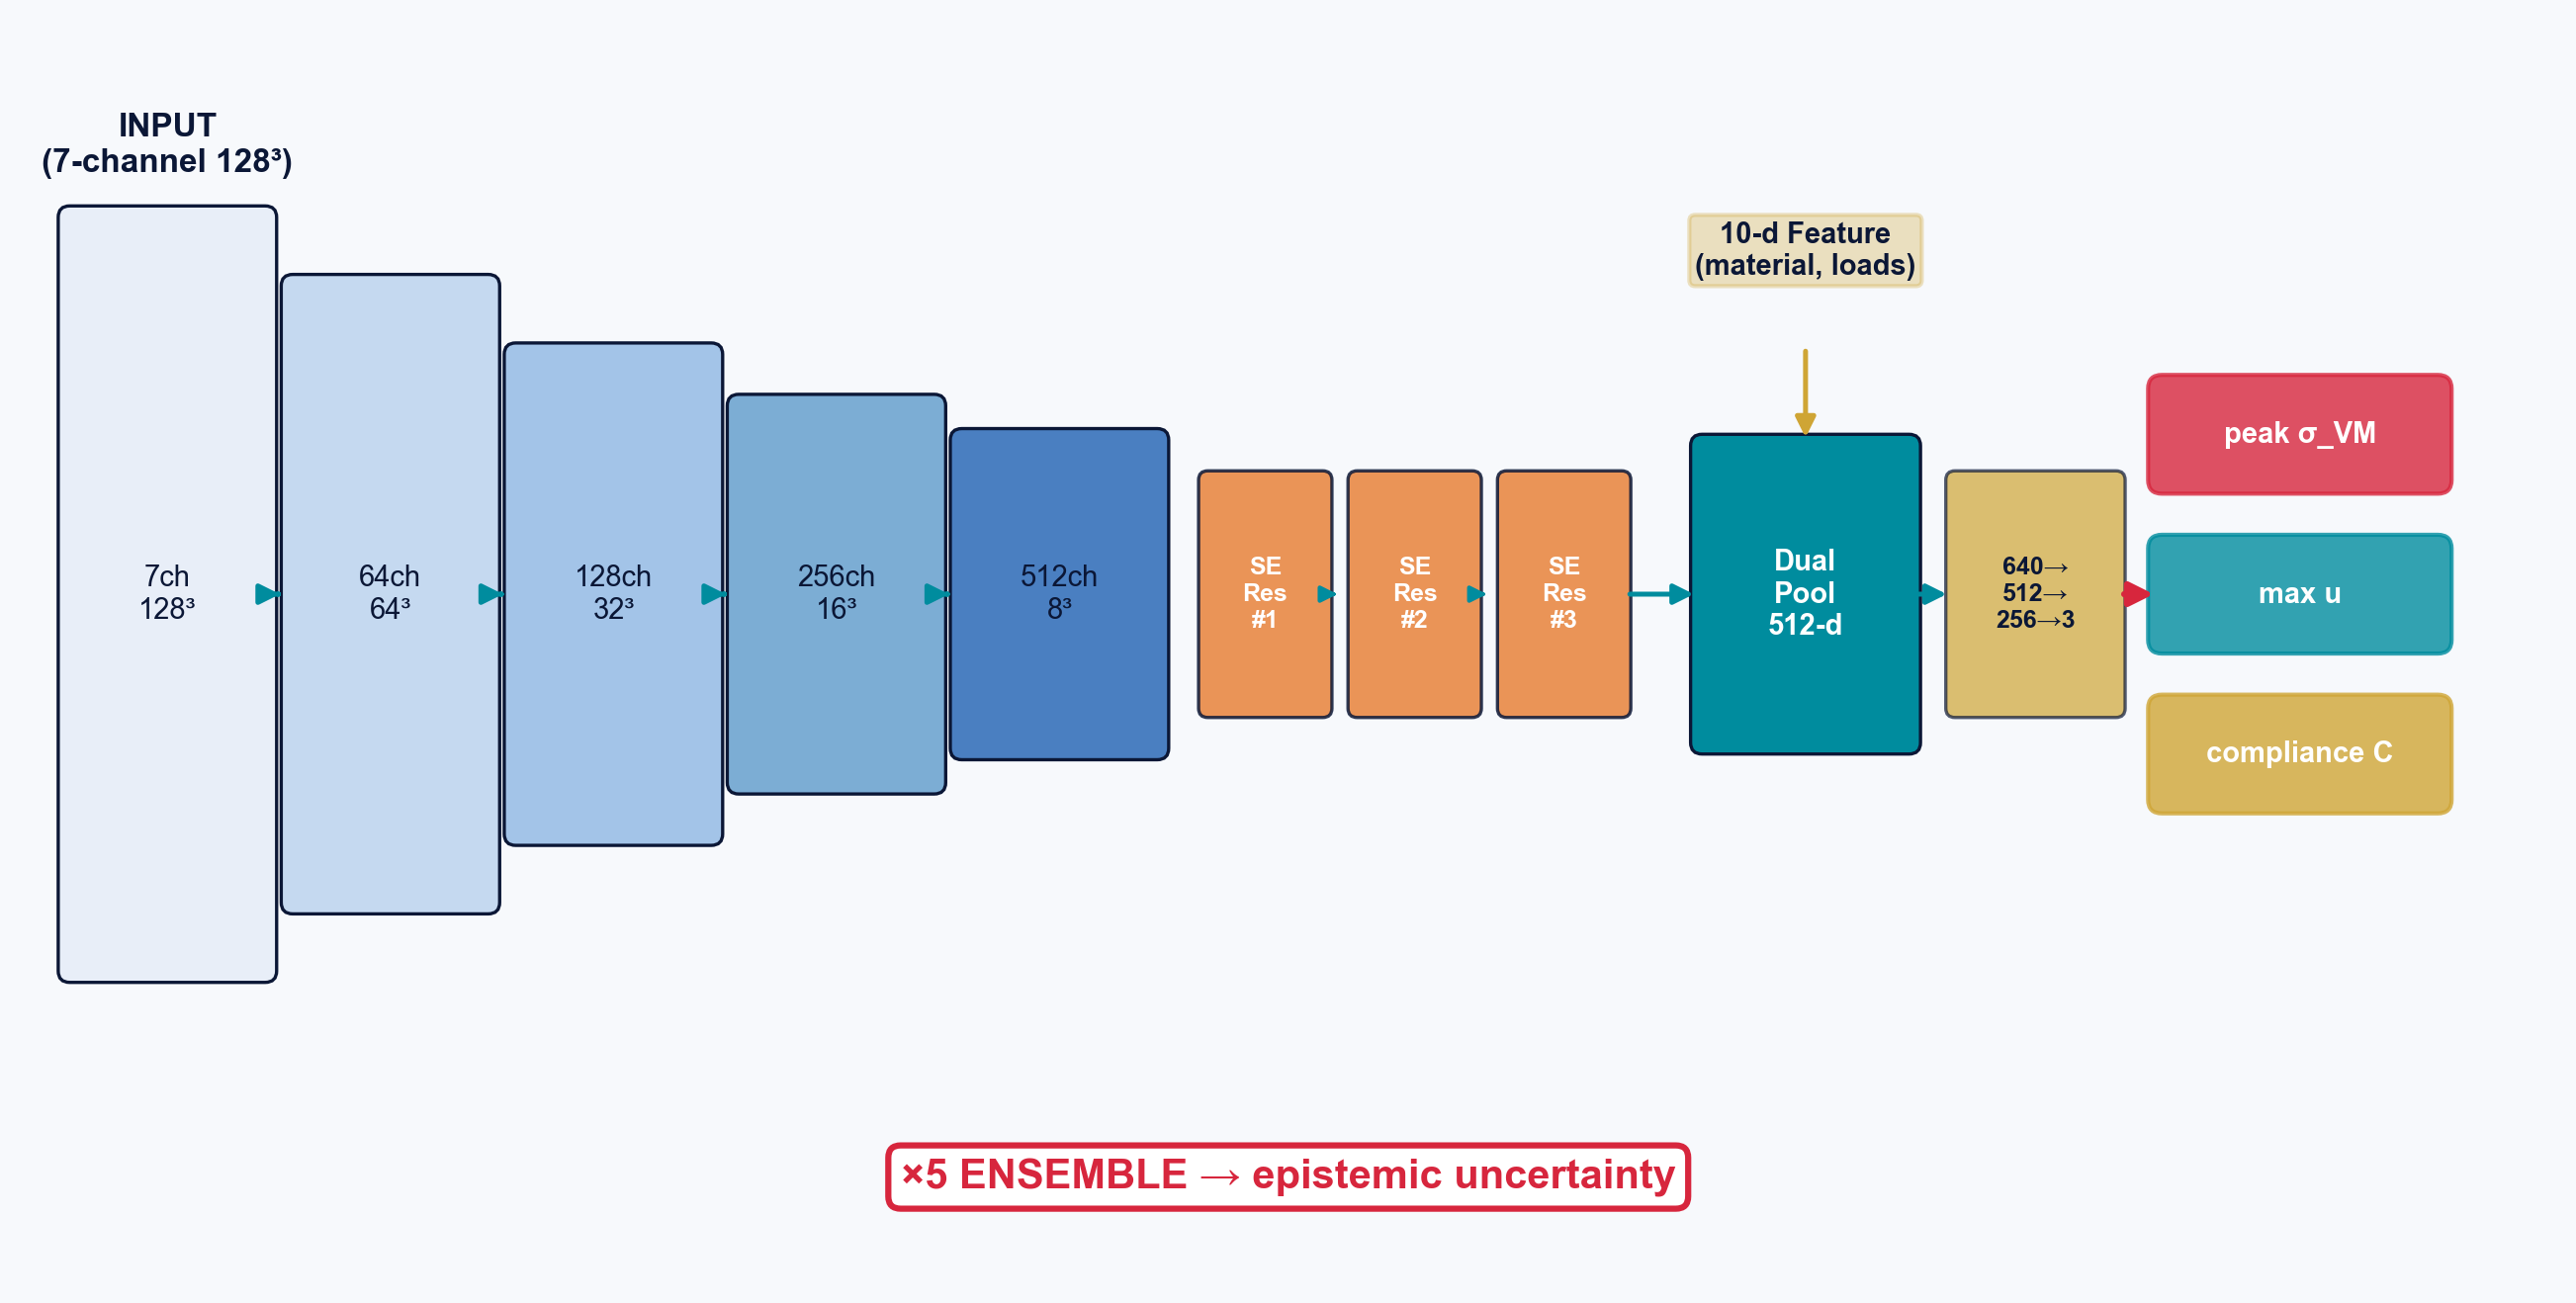
\includegraphics[width=\linewidth]{fig04_architecture.png}\\
{\captiontext Fig.~7. Single ensemble member architecture. Five independently trained members form the deep ensemble.}

\vspace{6pt}
\subheader{Topology Preservation: 6-Connectivity}
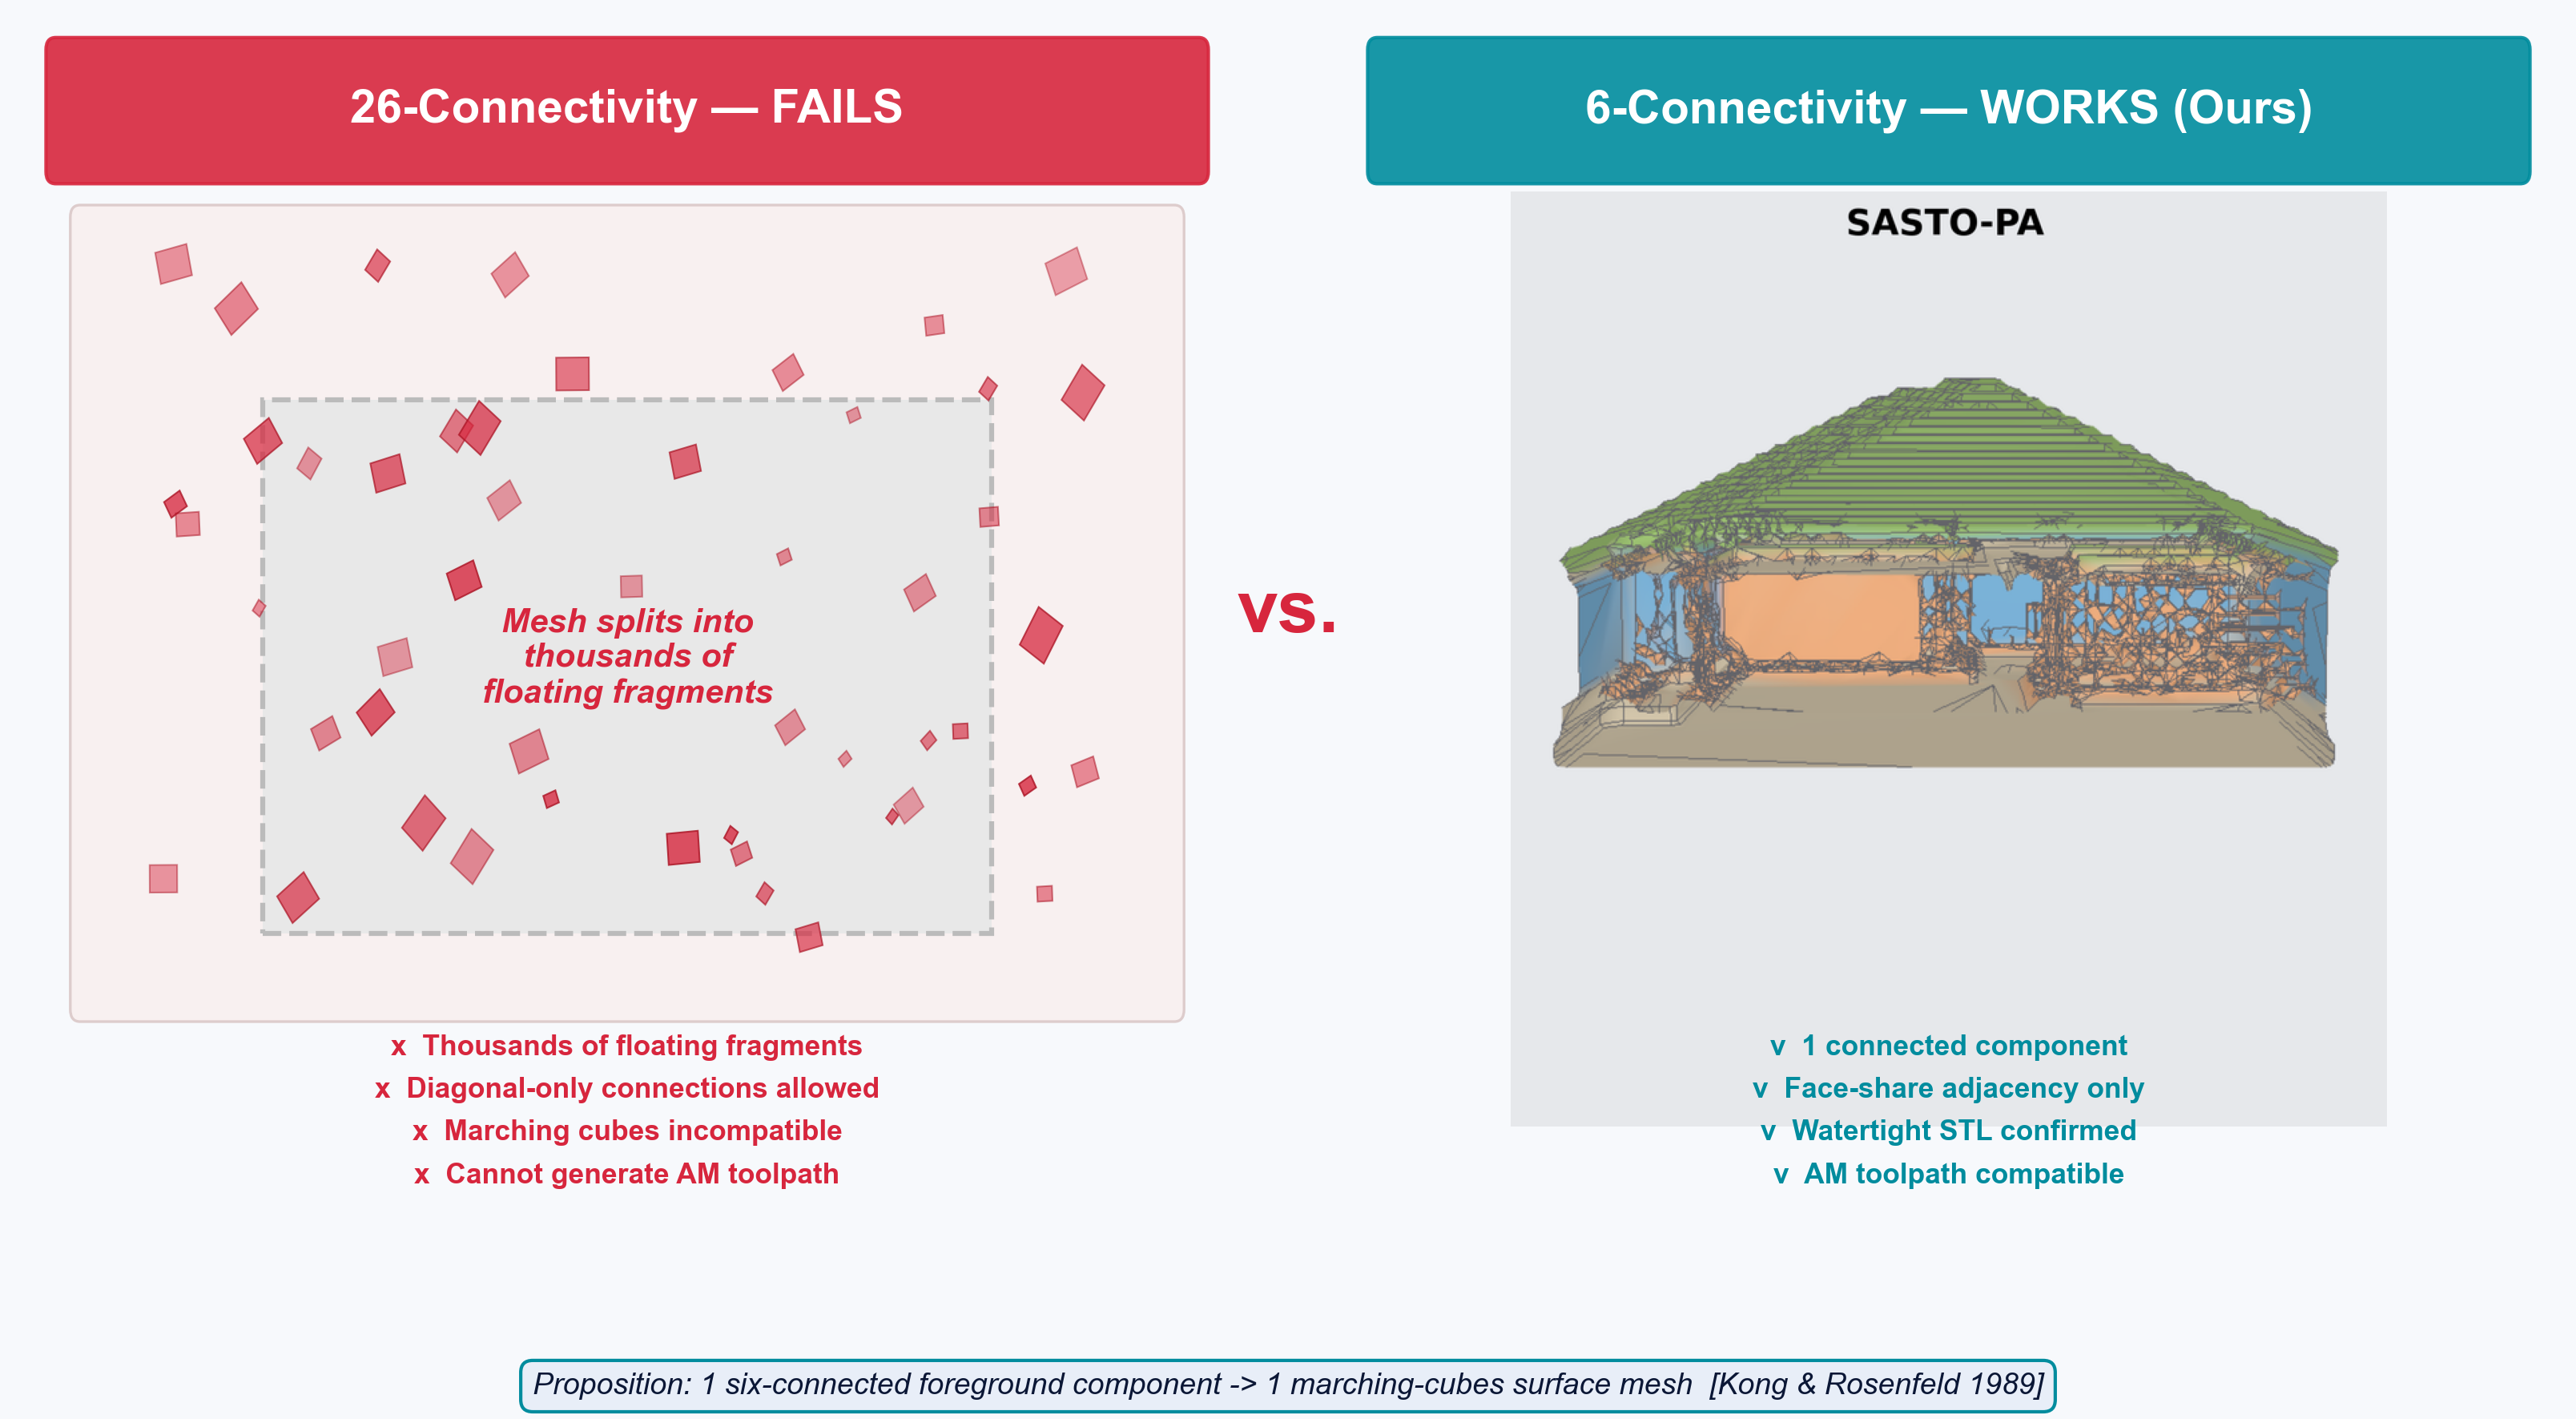
\includegraphics[width=\linewidth]{fig06_connectivity.png}\\
{\captiontext Fig.~9. The 6-connectivity criterion eliminates floating fragments incompatible with AM toolpath generation.}
\end{column}
\end{columns}
\end{sectionbox}

\vspace{4pt}

% ── C2: RESULTS & IN-SILICO VALIDATION ───────────────────────
\begin{sectionbox}{Results \& In-Silico Validation}
\bodytext

\begin{columns}[T]
% Col A: Reference Case
\begin{column}{0.31\textwidth}
\subheader{Reference Case (Sample 00472)}
% Before/after images would go here - use existing renders
{\captiontext [3D render: before/after optimization -- insert from screenshot\_stls/]}

\vspace{4pt}
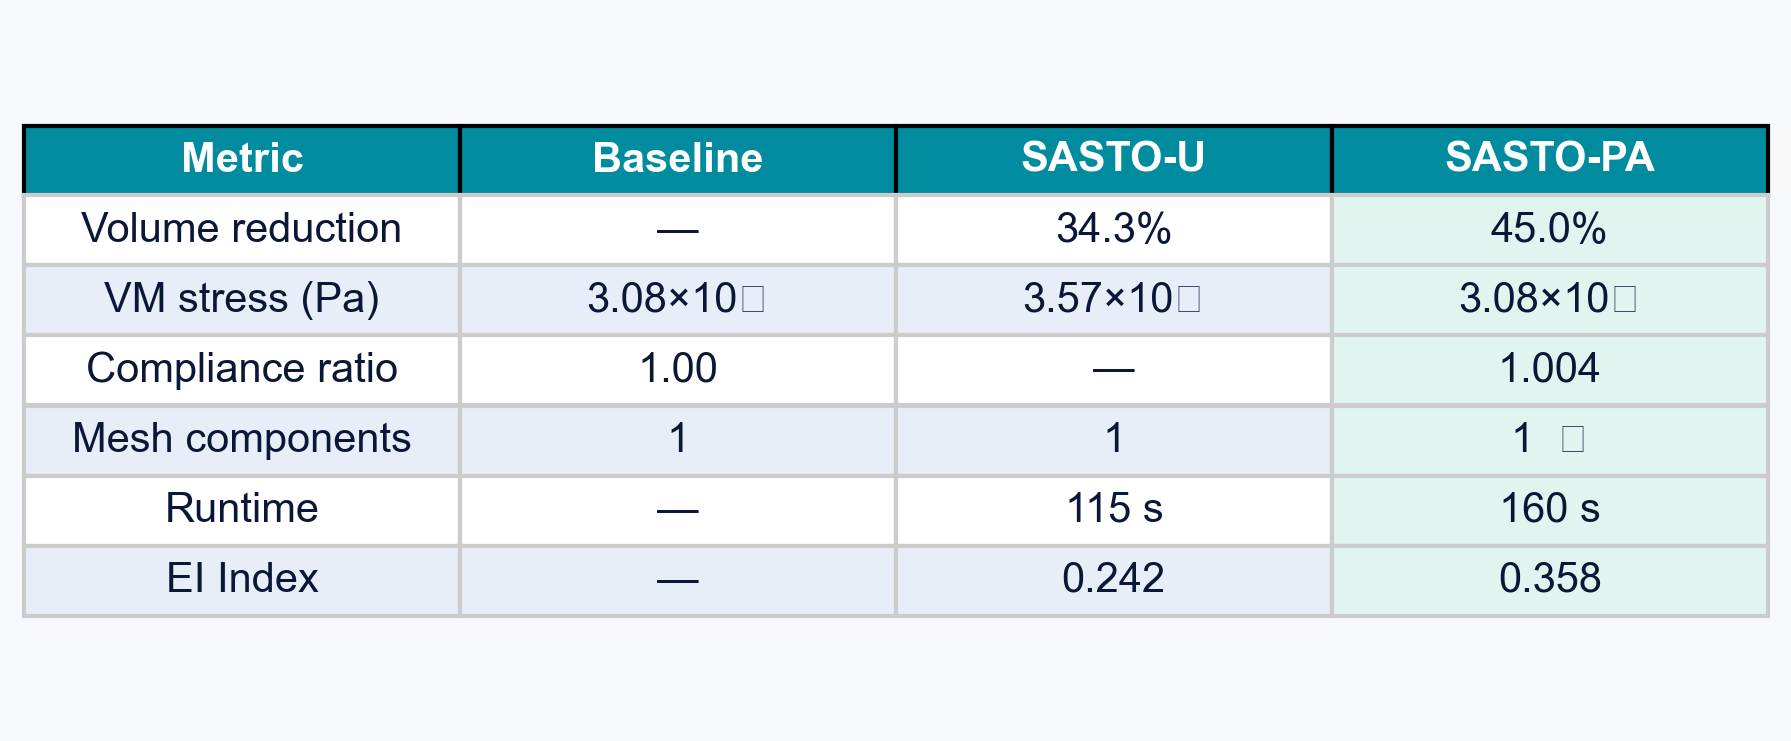
\includegraphics[width=\linewidth]{fig19_reference_table.png}\\
{\captiontext Table~1. Reference case: SASTO-PA achieves 10.7pp more reduction than SASTO-U.}
\end{column}

% Col B: Multi-Geometry
\begin{column}{0.31\textwidth}
\subheader{1,114-Geometry Generalization}
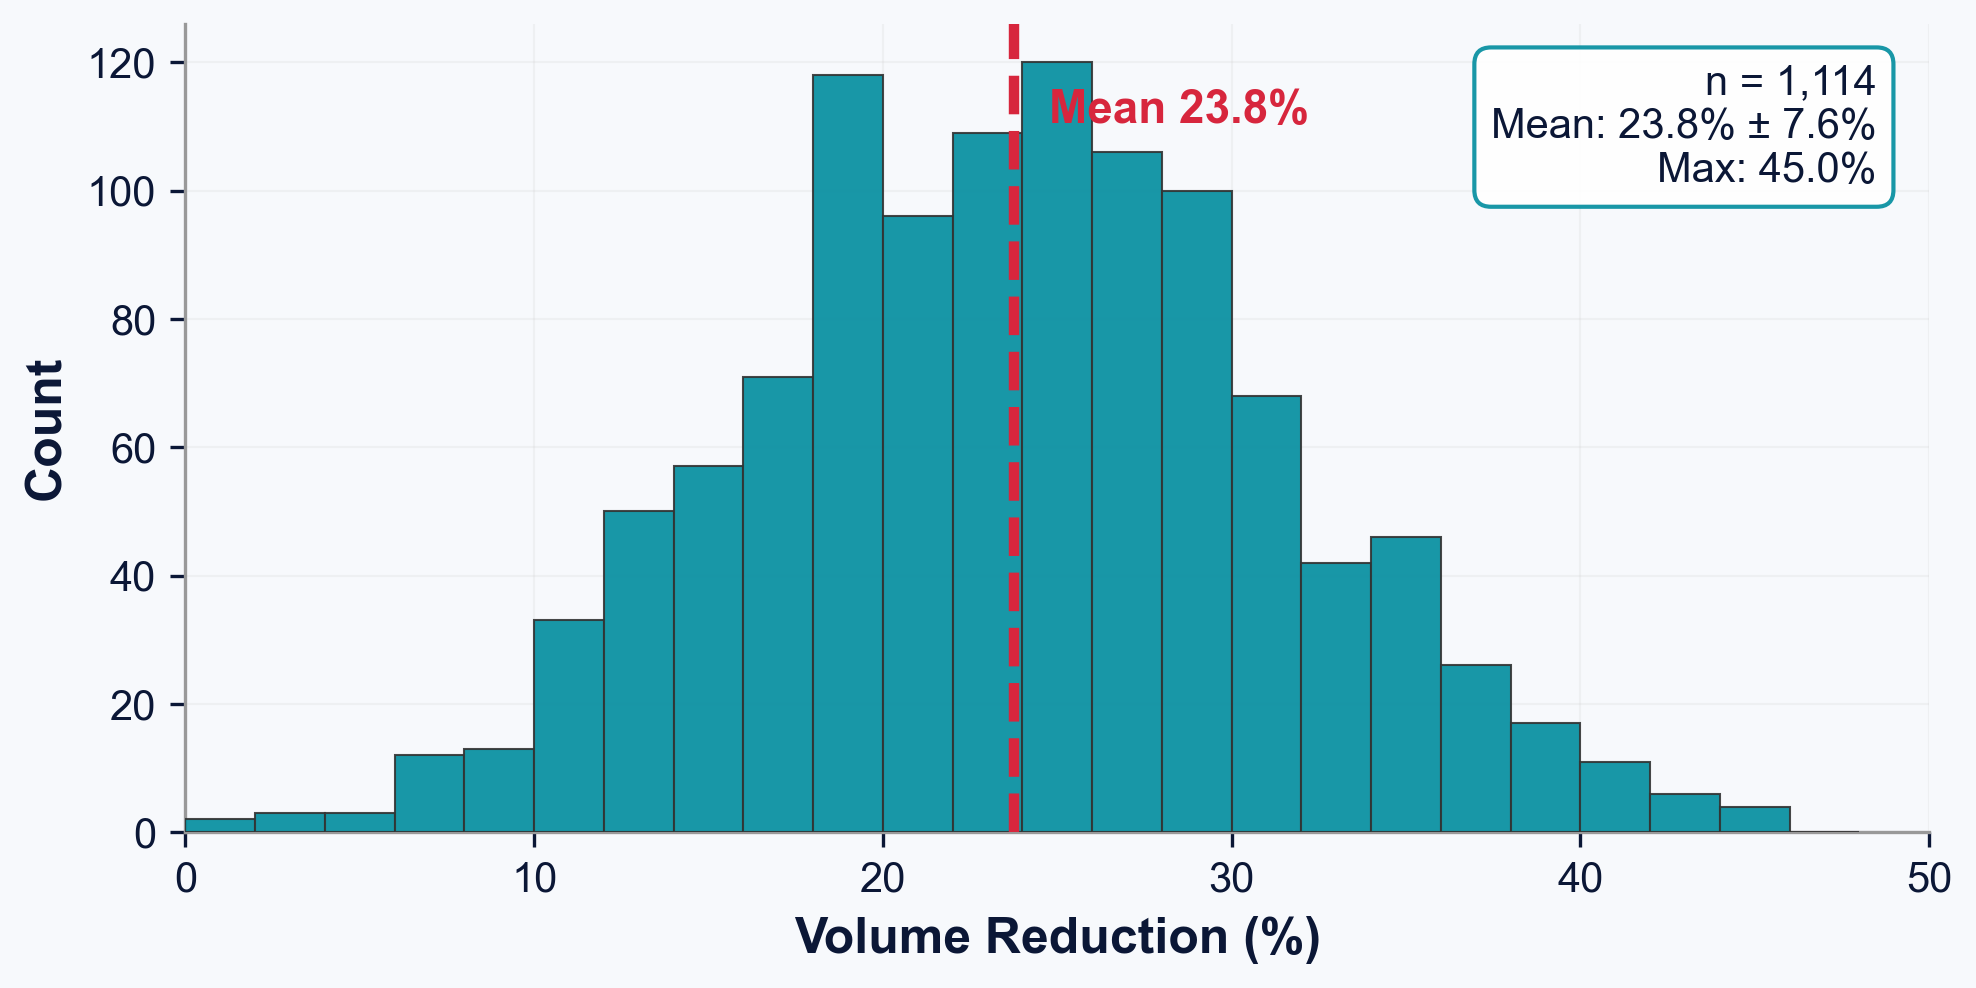
\includegraphics[width=\linewidth]{fig07_histogram.png}\\
{\captiontext Fig.~10. Volume reduction distribution across 1,114 held-out designs.}

\vspace{4pt}
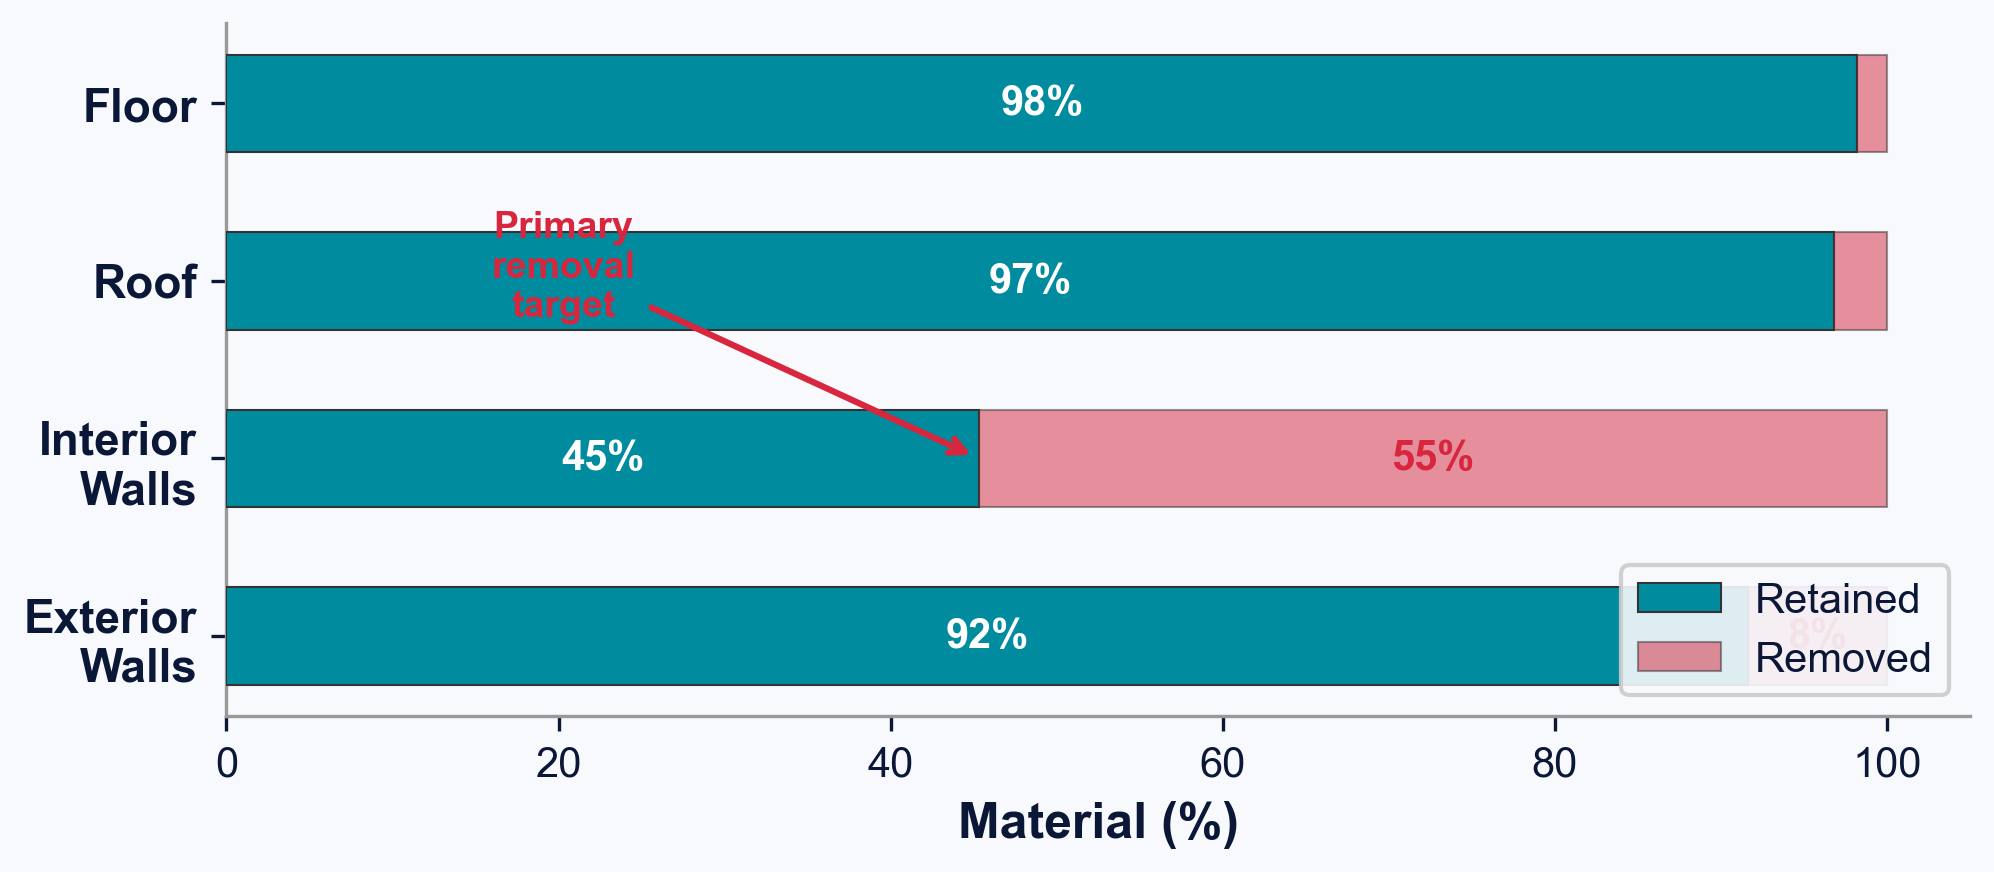
\includegraphics[width=\linewidth]{fig08_per_part.png}\\
{\captiontext Fig.~11. Per-part material retention. Interior walls: primary removal target.}
\end{column}

% Col C: Speedup & Validation
\begin{column}{0.31\textwidth}
\subheader{Speedup \& Independent Validation}
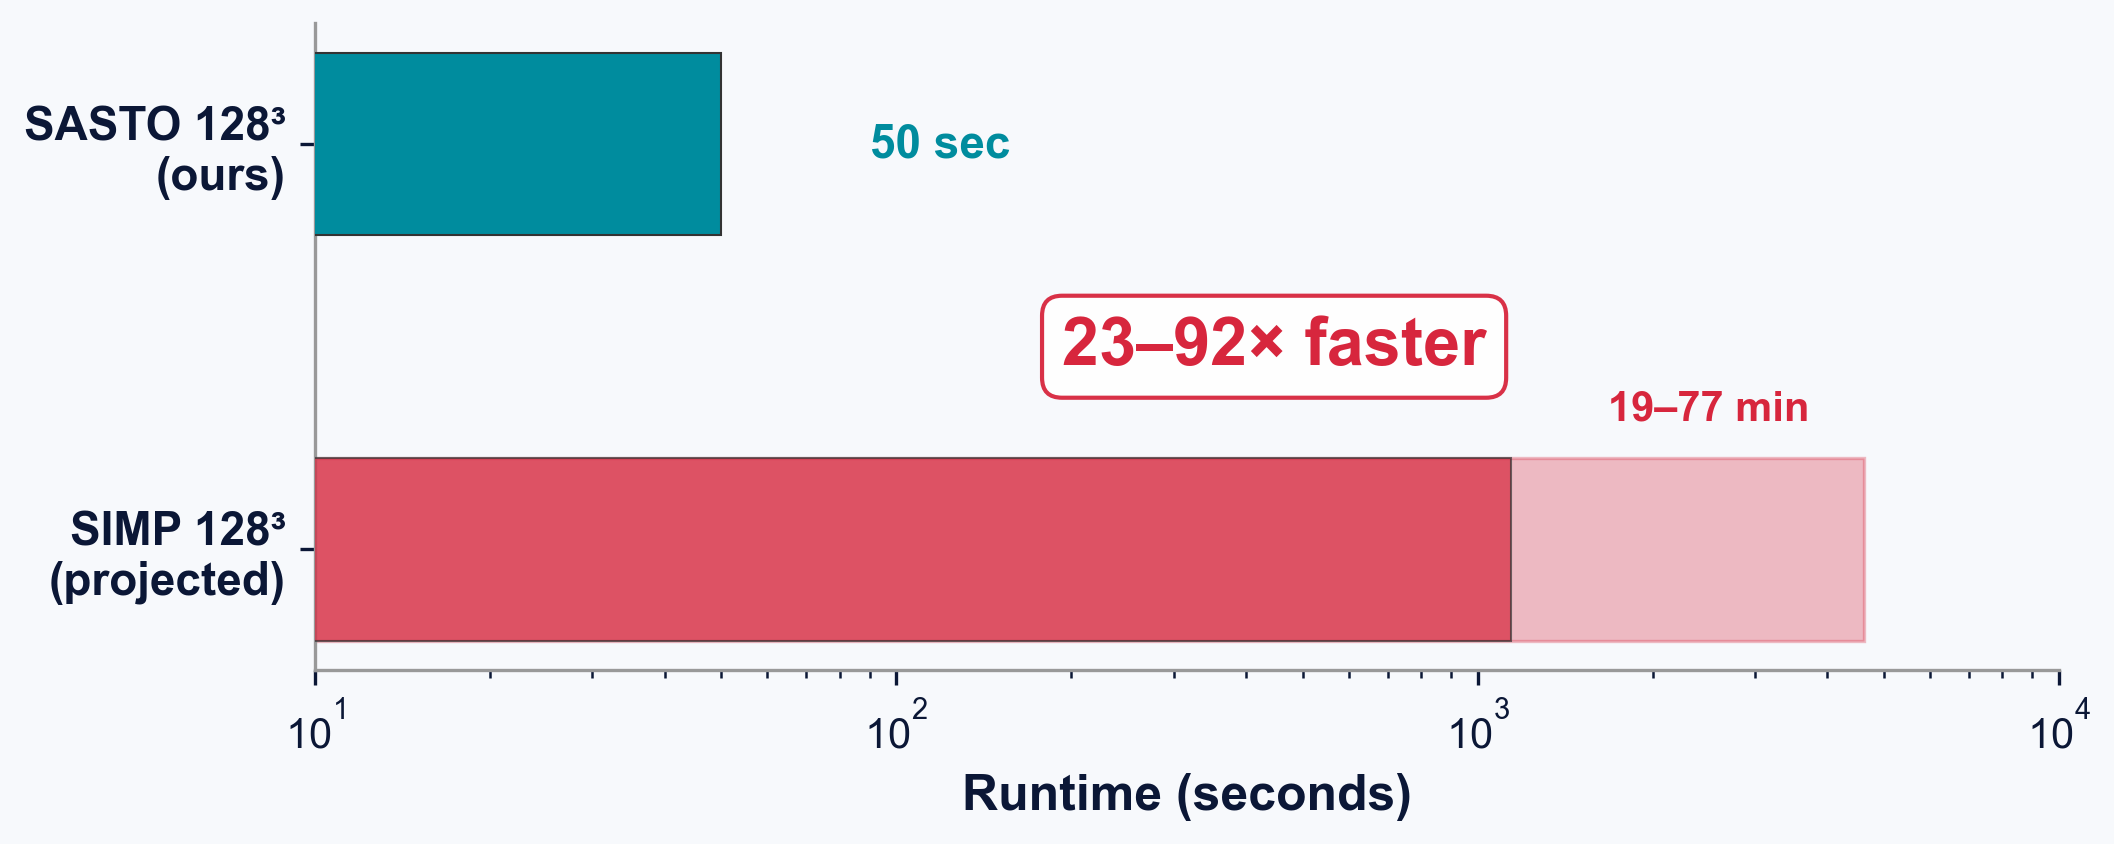
\includegraphics[width=\linewidth]{fig09_speedup.png}\\
{\captiontext Fig.~12. Even at 64$^3$, SIMP median 94s vs.\ SASTO 50s at 128$^3$.}

\vspace{4pt}
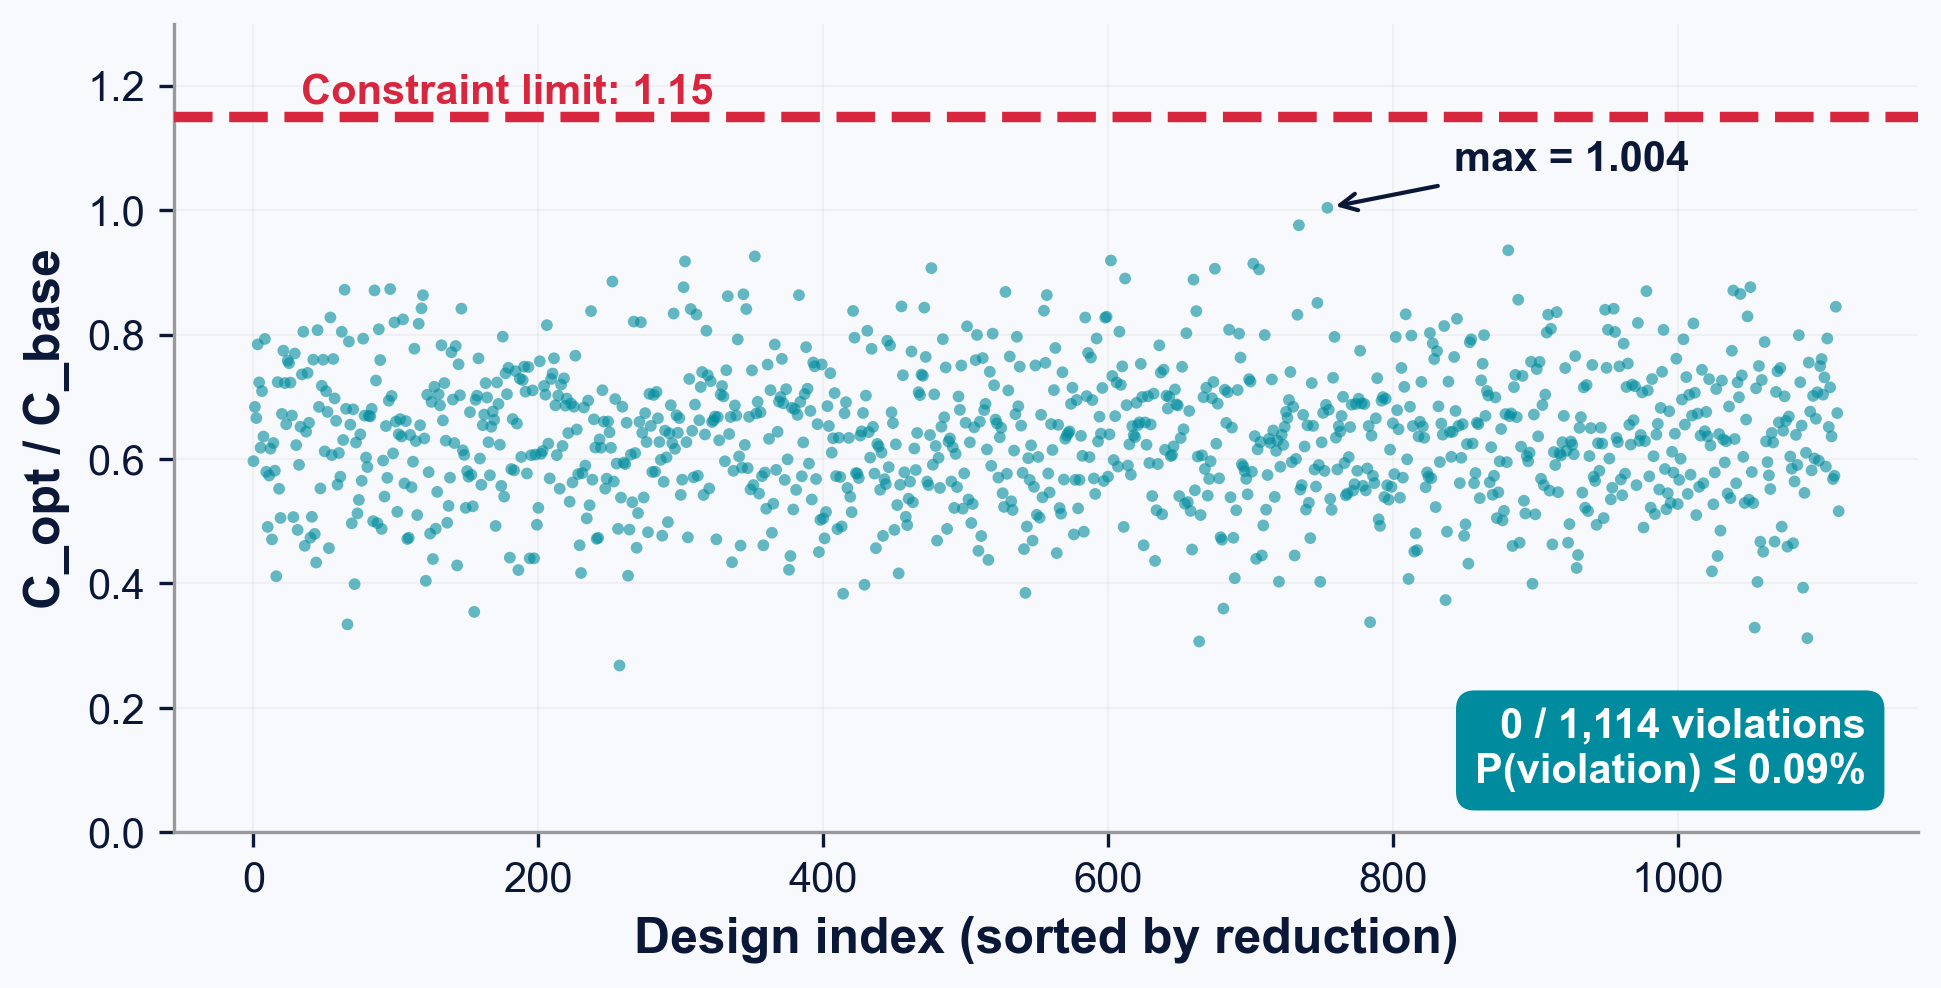
\includegraphics[width=\linewidth]{fig10_fea_compliance.png}\\
{\captiontext Fig.~13. Independent hex8 FEA re-analysis: 0/1,114 violations.}
\end{column}
\end{columns}

\vspace{8pt}

% KEY STATS BANNER
\centering

\includegraphics[width=\linewidth]{fig20_stats_banner.png}

\end{sectionbox}

\end{column}

% ══════════════════════════════════════════════════════════════
% RIGHT PANEL (12 inches = 30.48cm)
% ══════════════════════════════════════════════════════════════
\begin{column}{0.25\textwidth}

% ── R1: STATISTICAL ANALYSIS ─────────────────────────────────
\begin{sectionbox}{Statistical Analysis}
\bodytext

\subheader{Surrogate Model Performance}
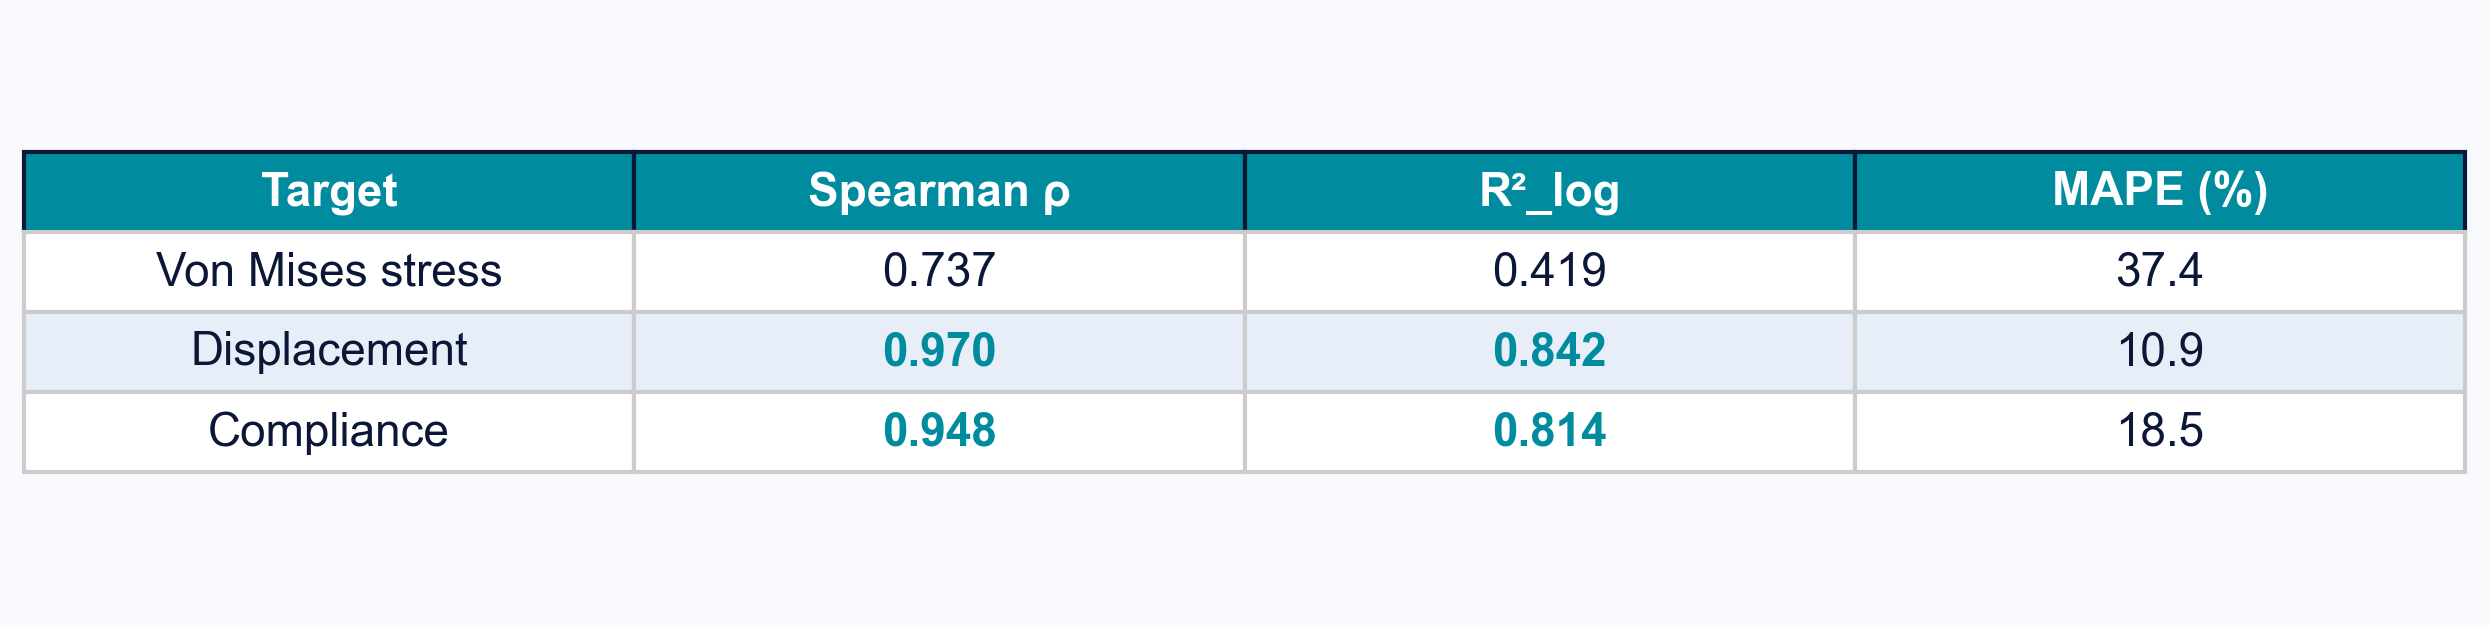
\includegraphics[width=\linewidth]{fig15_surrogate_table.png}\\
{\captiontext Surrogate requires ranking accuracy, not pointwise accuracy --- compliance Spearman $\rho = 0.948$ drives optimization safety.}

\vspace{4pt}
\subheader{Optimization Convergence}
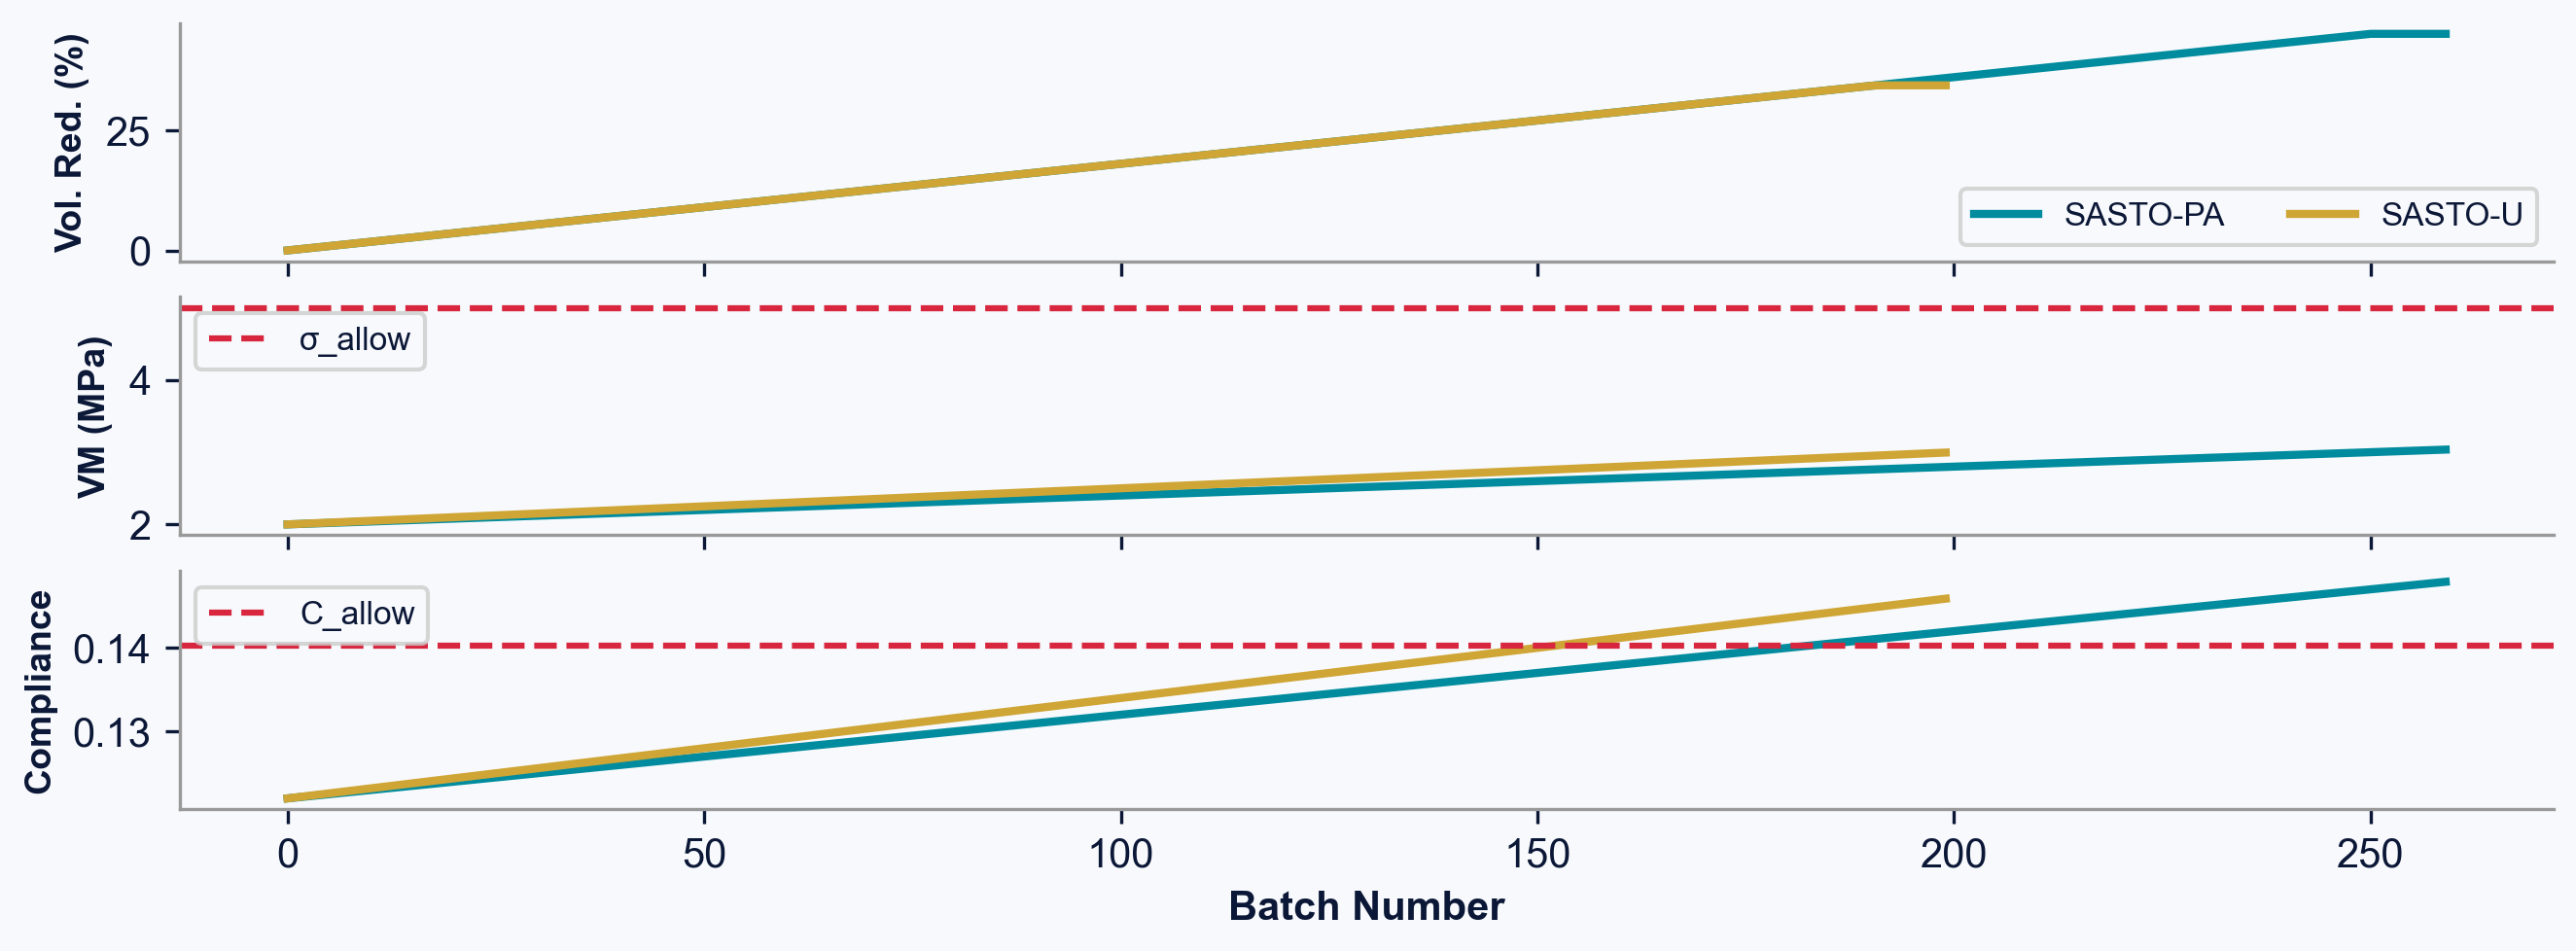
\includegraphics[width=\linewidth]{fig11_convergence.png}\\
{\captiontext Fig.~14. SASTO-PA (teal) removes more material than SASTO-U (gold) via part-aware thinning.}

\vspace{4pt}
\subheader{k-Factor Sensitivity}
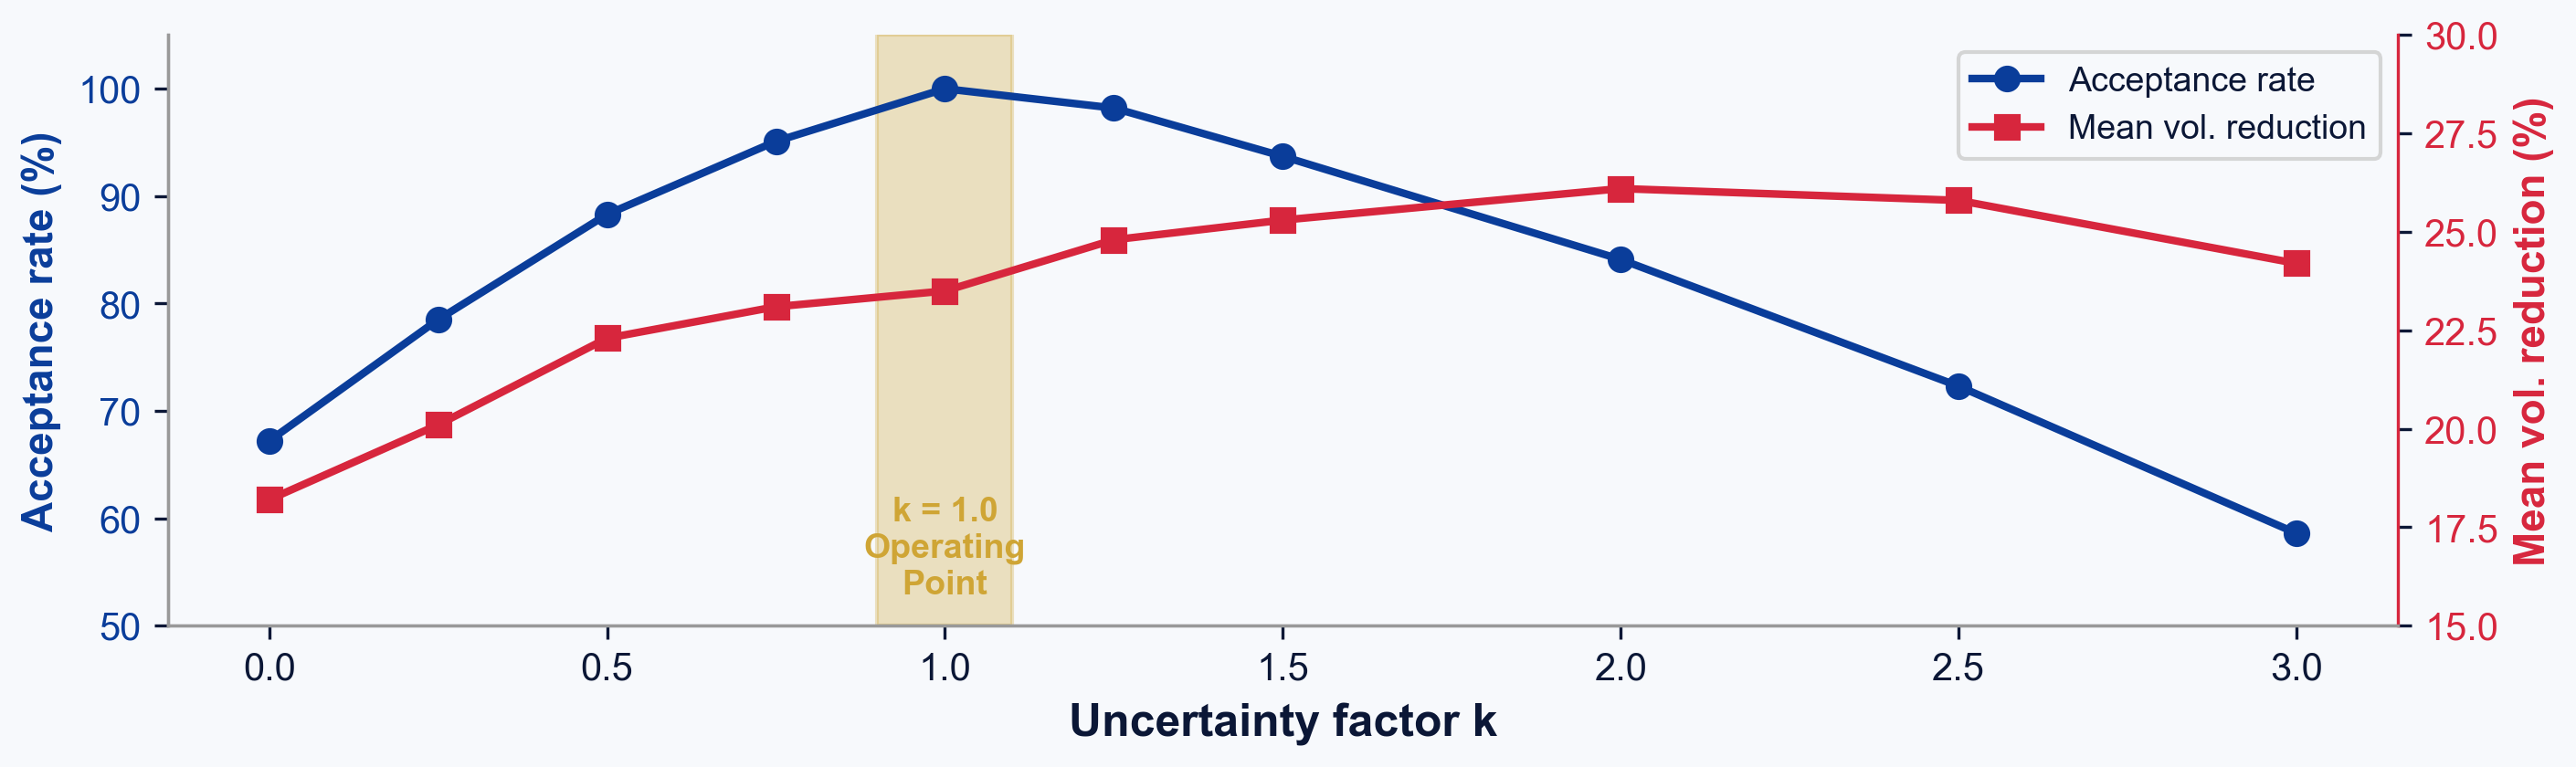
\includegraphics[width=\linewidth]{fig12_k_factor.png}\\
{\captiontext Fig.~15. k-factor ablation: 100\% acceptance at $k = 1.0$ is by construction.}

\vspace{4pt}
\subheader{Conformal Prediction Calibration}
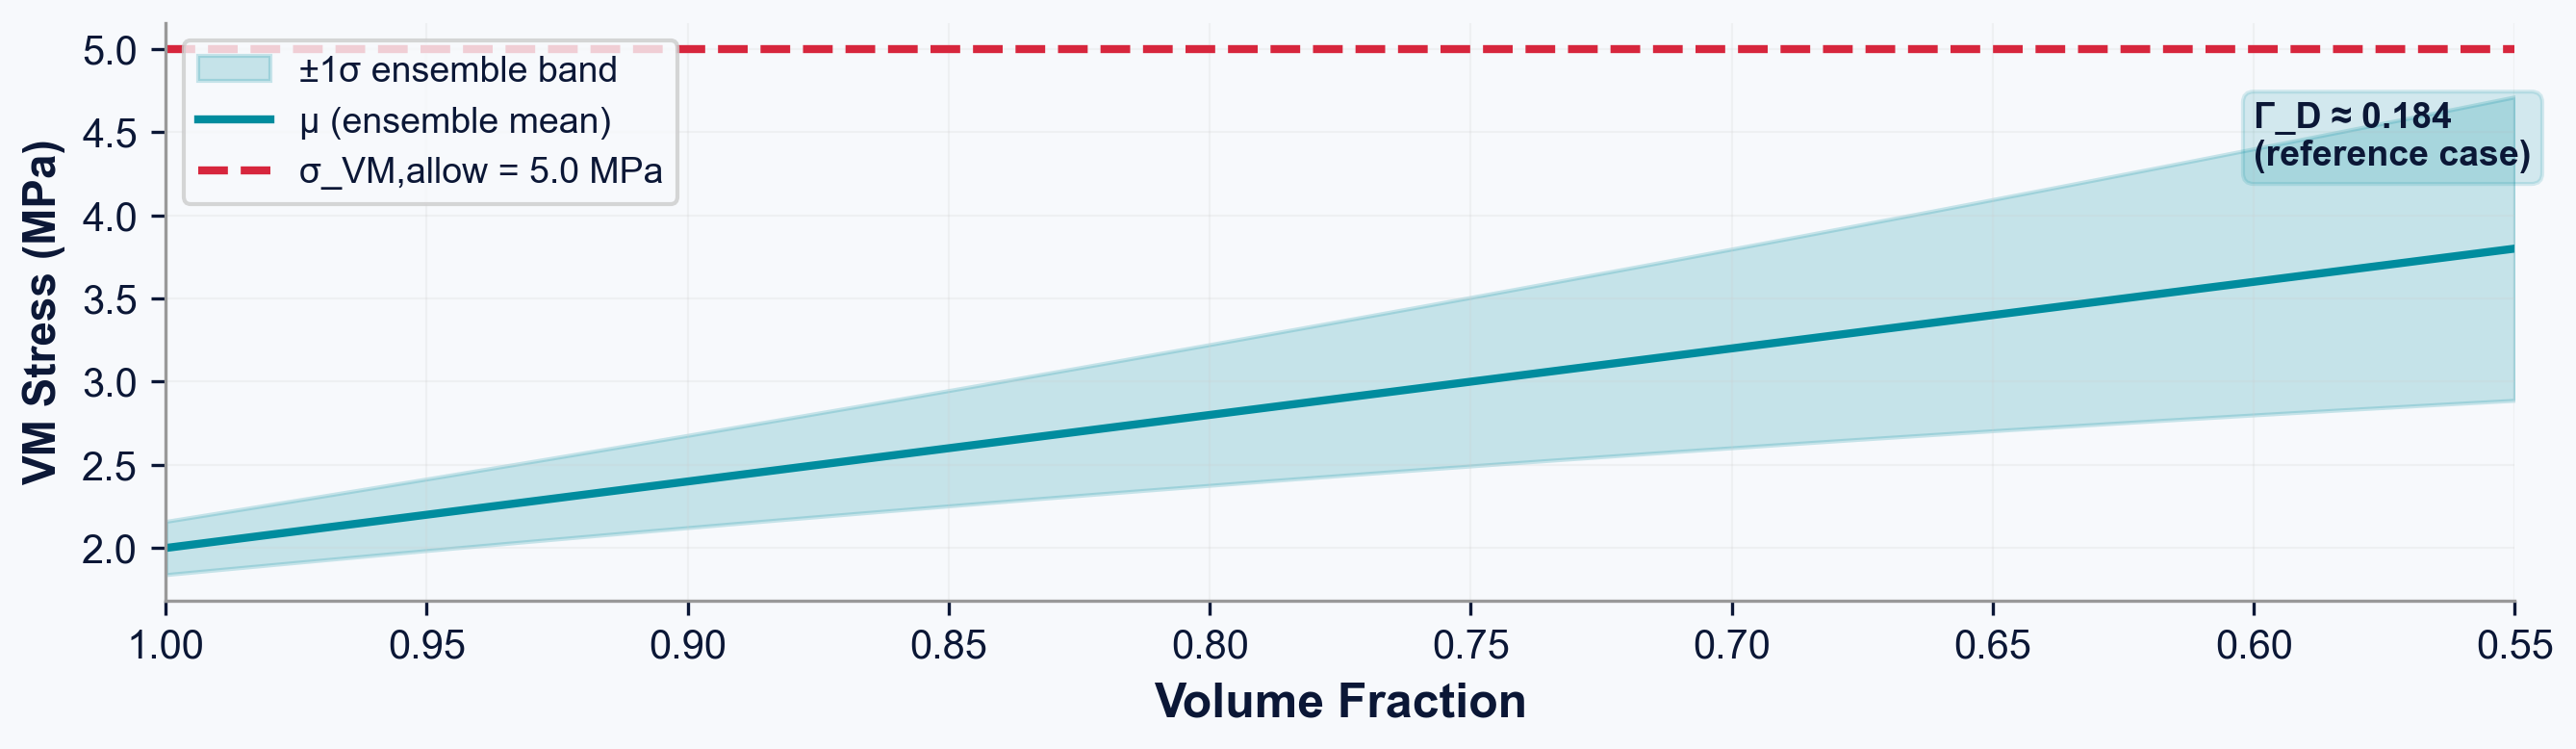
\includegraphics[width=\linewidth]{fig13_uncertainty.png}\\
{\captiontext Fig.~16. Ensemble uncertainty bands. $\Gamma_D \approx 0.184$ confirms sub-linear uncertainty growth.}

\vspace{4pt}
\begin{eqbox}
\centering
{\small SASTO achieves $R^2_{\log} = 0.814$ for compliance.\\
$\Gamma_D = 0.255$ mean across 1,114 designs.\\
$P(\text{violation}) \le 0.09\%$ (conformal, $n = 1{,}114$, distribution-free).}
\end{eqbox}
\end{sectionbox}

\vspace{4pt}

% ── R2: CONCLUSIONS ──────────────────────────────────────────
\begin{sectionbox}{Conclusions}
\bodytext

\begin{enumerate}[leftmargin=*, itemsep=4pt, label={\color{accentteal}\bfseries\arabic*.}]
    \item SASTO achieves \textbf{23.5\% $\pm$ 7.8\%} mean material reduction across 1,114 held-out designs, up to 45.0\% on individual houses, with all proxy structural constraints satisfied.
    \item The deep ensemble surrogate provides a \textbf{23--92$\times$} empirically-anchored speedup vs.\ SIMP, running in a median \textbf{50 seconds} on a consumer laptop GPU.
    \item The \textbf{6-connectivity criterion} eliminates floating mesh fragments, guaranteeing watertight single-component STL meshes for every optimized design.
    \item \textbf{Part-aware thickness} yields 10.7pp more reduction than uniform thickness by permitting 1-voxel interior walls.
    \item Independent FEA re-analysis confirms \textbf{zero violations} ($\max C_\mathrm{opt}/C_\mathrm{base} = 1.004$). Conformal prediction certifies $P(\text{violation}) \le 0.09\%$.
\end{enumerate}

\vspace{4pt}
\begin{eqbox}
\centering
{\small 8\% of global CO\textsubscript{2} = cement production. 23.5\% less concrete per house $\to$ potential for millions of tons saved at scale.}
\end{eqbox}
\end{sectionbox}

\vspace{4pt}

% ── R3: FUTURE WORK ──────────────────────────────────────────
\begin{sectionbox}{Future Work}
\bodytext

\begin{enumerate}[leftmargin=*, itemsep=3pt, label={\color{accentteal}\bfseries\arabic*.}]
    \item \textbf{FEA-in-the-Loop Active Learning:} When ensemble disagreement $\Gamma_D$ exceeds threshold $\tau$, trigger a ground-truth FEA solve mid-optimization. Creates self-correcting safety net.
    \item \textbf{Nonlinear FEA Spot Checks:} For 5 representative designs, run concrete damaged plasticity (CDP) to assess cracking or buckling invisible to the linear surrogate.
    \item \textbf{Physical Print Validation:} Fabricate one optimized house at 1:10 scale. Compression testing + DIC full-field strain measurement vs.\ model predictions.
\end{enumerate}
\end{sectionbox}

\vspace{4pt}

% ── R4: KEY REFERENCES ────────────────────────────────────────
\begin{sectionbox}{Key References}
{\fontsize{11}{13}\selectfont\color{textdark}

\begin{enumerate}[leftmargin=*, itemsep=1pt, label={\arabic*.}]
    \item Bends{\o}e \& Sigmund (2003). \textit{Topology Optimization}. Springer.
    \item Lakshminarayanan et al.\ (2017). Deep ensembles. \textit{NeurIPS}.
    \item Kong \& Rosenfeld (1989). Digital topology. \textit{CVGIP} 48(3).
    \item ASCE (2022). \textit{ASCE/SEI 7-22}. ASCE.
    \item Buswell et al.\ (2018). 3D printing concrete. \textit{Cem.\ Concr.\ Res.}\ 112.
    \item Sigmund \& Maute (2013). Topology optimization. \textit{Struct.\ Multidisc.\ Optim.}\ 48.
    \item Lin et al.\ (2024). 3DWire dataset. KAUST VCC.
    \item IEA (2021). \textit{Global Status Report for Buildings}. IEA.
    \item Lorensen \& Cline (1987). Marching Cubes. \textit{SIGGRAPH}.
    \item Vovk et al.\ (2005). \textit{Algorithmic Learning in a Random World}. Springer.
\end{enumerate}
}
\end{sectionbox}

\end{column}

\end{columns}
\end{frame}
\end{document}
